\subsection{Figuras}

\begin{frame}
\epigraph{I call our world Flatland, not because we call it so, 
but to make its nature clearer to you, my happy readers, 
who are privileged to live in space.}{Edwin A. Abbott, Flatland: A Romance of Many Dimensions}
\end{frame}


\begin{frame}
\frametitle{Figuras}
Figuras possuem uma grande potencial para levar informação de forma simples ao leitor.
Podem evidenciar padrões, tendências e anomalias, constâncias ou variações. 
Devem ser utilizadas com parcimônia e muito bem elaboradas.

\vspace{3ex}
Figuras são elementos flutuantes e que devem ser capazes de passar uma mensagem sozinhas.
\end{frame}


\begin{frame}
\frametitle{xkcd}
\begin{figure}[h]
\centering
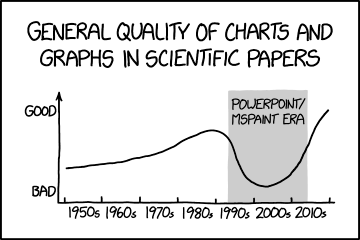
\includegraphics[width=0.6\textwidth,height=0.6\textheight,keepaspectratio]{figures/scientific_paper_graph_quality.png}
\caption{Scientific Paper Graph Quality (\url{https://xkcd.com/1945/}).}
\label{fig-scientific_paper_graph_quality}
\end{figure}
\end{frame}

\begin{frame}
\frametitle{Eventos na história da visualização de dados}
\begin{figure}[h]
\centering
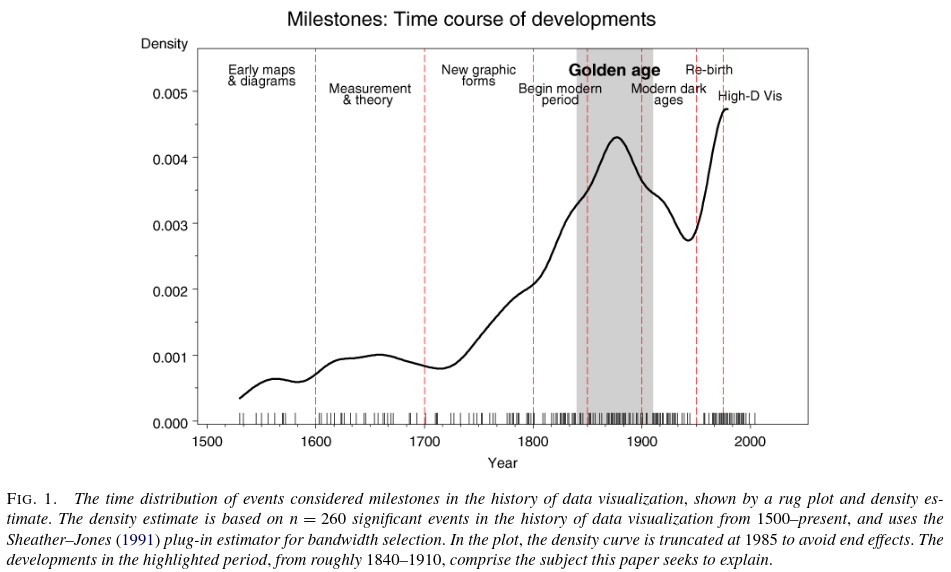
\includegraphics[width=0.8\textwidth,height=0.8\textheight,keepaspectratio]{figures/hist_data_visualization.png}
\caption{Retirada de \textcite{Friendly2008}.}
\label{fig-hist_data_visualization}
\end{figure}
\end{frame}


\begin{frame}
\frametitle{Figuras}

Florence Nightingale liderou uma pequena equipe de enfermeiras a Istambul em
1854 para ajudar no cuidado dos soldados britânicos que lutaram na guerra da
Crimeia. Seus gráficos convenceram os grandes e os bons de que as mortes devido
à sujeira e ao saneamento deficiente poderiam ser evitadas - salvando inúmeras
vidas.

\vspace{2ex}
\fullcite{harford_florence}

\vspace{1ex}
\hrefcolor{https://99percentinvisible.org/episode/florence-nightingale-data-viz-pioneer/}{Florence Nightingale: Data Viz Pioneer, 99percentinvisible.org}

\hrefcolor{https://en.wikipedia.org/wiki/Florence_Nightingale}{Florence Nightingale, Wikipedia}

\hrefcolor{https://www.youtube.com/watch?v=VTdVPNvwULM}{Nightingale Diagrams, Numberphile}

\hrefcolor{https://www.youtube.com/watch?v=sNppKQh0xPo}{What would Florence Nightingale make of big data?, BBC Ideas}
\end{frame}
% Coxcomb plots and 'spiecharts' in R
% https://rpubs.com/RobinLovelace/11641

\begin{frame}
\frametitle{Florence Nightingale}
\begin{figure}[h]
 \centering
 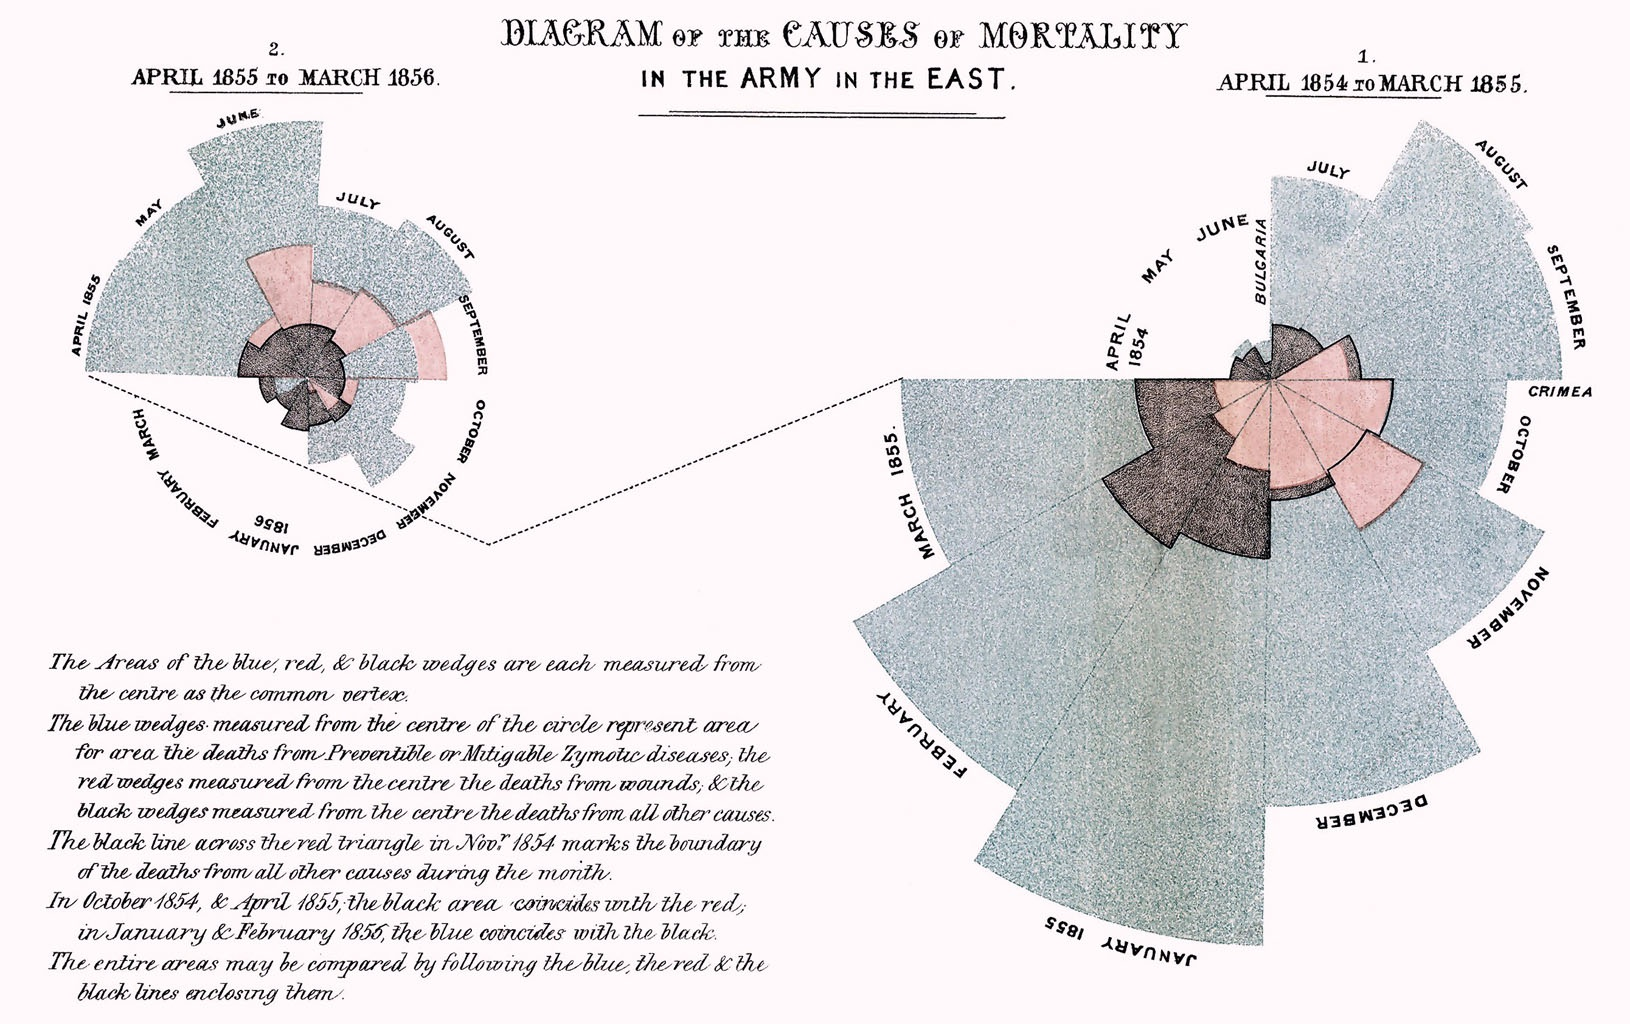
\includegraphics[width=0.8\textwidth,height=0.75\textheight,keepaspectratio]{figures/nightingale-mortality.jpg}
 \caption{Diagrama de mortalidade feito por Florence Nightingale.}
 \label{fig-nightingale-mortality}
\end{figure}
\end{frame}
\note{
O gráfico proposto por Florence Nightingale evidencia as mortes pelas áreas, sendo
dividas por três causas: doenças infectocontagiosas (azul), ferimentos (vermelho) e outras (preto).
O gráfico da direito apresenta o período durante a guerra antes da adoção de medidas sanitárias
e o gráfico da esquerda evidencia o período após a adoções de medidas sanitárias. 
O tempo é visto no sentido horário e a posição no gráfico facilita a comparação dos
meses em anos diferentes.
}






\begin{frame}[allowframebreaks]
\frametitle{Exemplo 1 - \emph{Storytelling with Data}}
\begin{figure}[h]
 \centering
 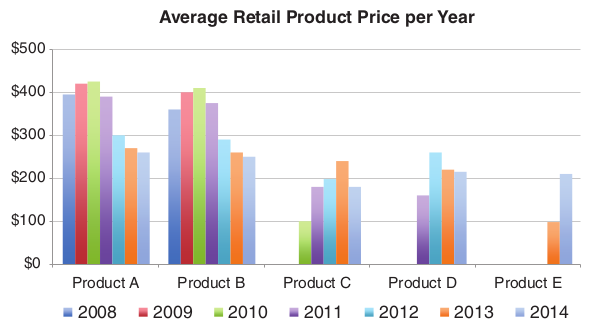
\includegraphics[width=0.8\textwidth,height=0.6\textheight,keepaspectratio]{figures/storytelling_data_ex01a.png}
 \caption{Preço médio de venda de produtos ao longo dos anos \cite{knaflic_storytelling_2015}.}
 \label{fig-storytelling_data_ex01a}
\end{figure}
\framebreak
\begin{figure}[h]
 \centering
 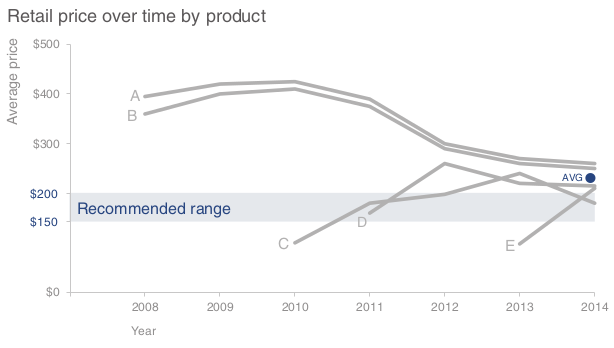
\includegraphics[width=0.8\textwidth,height=0.7\textheight,keepaspectratio]{figures/storytelling_data_ex01b.png}
 \caption{Preço médio de venda de produtos ao longo dos anos \cite{knaflic_storytelling_2015}.}
 \label{fig-storytelling_data_ex01b}
\end{figure}
\end{frame}


\begin{frame}[allowframebreaks=1]
\frametitle{Exemplo 2 - \emph{Storytelling with Data}}
\begin{figure}[h]
 \centering
 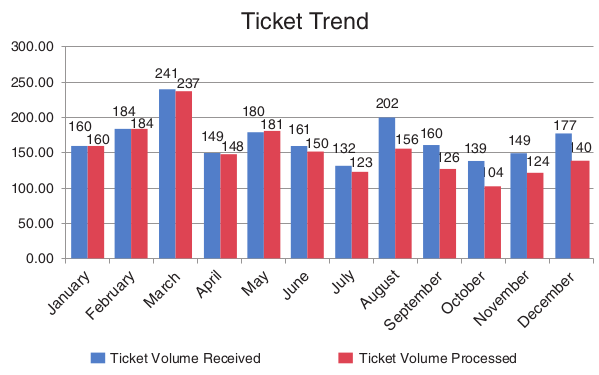
\includegraphics[width=0.8\textwidth,height=0.6\textheight,keepaspectratio]{figures/storytelling_data_ex02a.png}
 \caption{Volume de tickes recebidos e processados. \cite{knaflic_storytelling_2015}.}
 \label{fig-storytelling_data_ex02a}
\end{figure}
\framebreak
\begin{figure}[h]
 \centering
 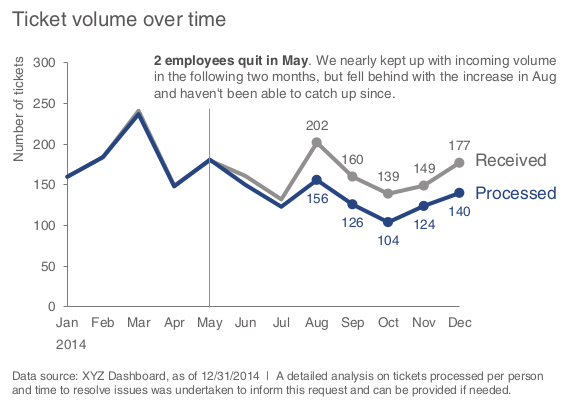
\includegraphics[width=0.8\textwidth,height=0.7\textheight,keepaspectratio]{figures/storytelling_data_ex02b.png}
 \caption{Volume de tickes recebidos vs. processados. O descolamento evidencia a necessidade de contratação. \cite{knaflic_storytelling_2015}.}
 \label{fig-storytelling_data_ex02b}
\end{figure}
\end{frame}

\begin{frame}[allowframebreaks=1]
\frametitle{Exemplo 3 - \emph{Storytelling with Data}}
\begin{figure}[h]
 \centering
 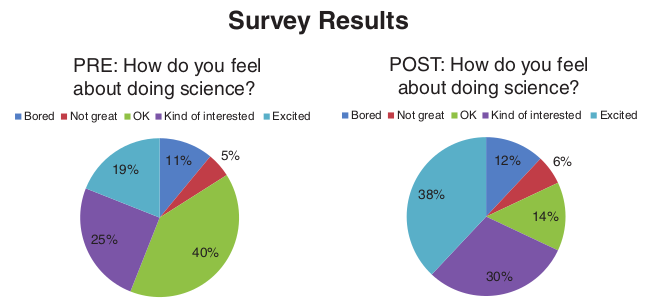
\includegraphics[width=0.8\textwidth,height=0.6\textheight,keepaspectratio]{figures/storytelling_data_ex03a.png}
 \caption{Resultado da pesquisa de opinião sobre ciências. \cite{knaflic_storytelling_2015}.}
 \label{fig-storytelling_data_ex03a}
\end{figure}
\framebreak
\begin{figure}[h]
 \centering
 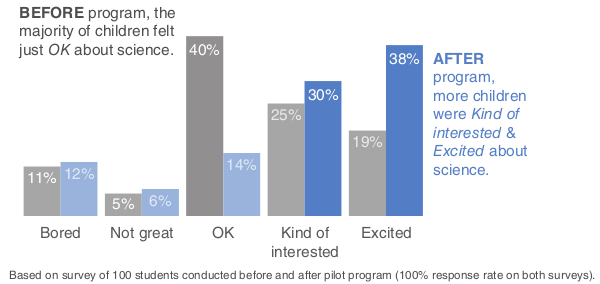
\includegraphics[width=0.7\textwidth,height=0.6\textheight,keepaspectratio]{figures/storytelling_data_ex03b.png}
 \caption{Resultado da pesquisa de opinião sobre ciências. \cite{knaflic_storytelling_2015}.}
 \label{fig-storytelling_data_ex03b}
\end{figure}
\end{frame}


\begin{frame}[allowframebreaks,fragile]
\frametitle{Limitações de alguns gráficos}

\begin{lstlisting}[language=Octave, label=lst-pie-ex, caption={Exemplo de limitações do gráficos.}, postbreak=\mbox{$\hookrightarrow$\space}, basicstyle=\fontsize{8}{10}\selectfont\ttfamily]
x = [0.07 0.12 0.08 0.13 0.075 0.126 0.083 0.135 0.063 0.118]; 
pie(x,strcat('item',strsplit(num2str(1:length(x)))));
print -dsvg piex.svg

lbs=strcat('item',strsplit(num2str(1:length(x))));
[_,idx]=sort(x);
pie(x(idx),lbs(idx)); 

plot(x,'ok','markerfacecolor','k')
set(gca,'Visible','off')
axes('Position',get(gca,'Position'),'XAxisLocation','bottom','YAxisLocation','left', 'Color','none','XTickLabel',get(gca,'XTickLabel'),'YTickLabel',get(gca,'YTickLabel'),'XColor','k','YColor','k','LineWidth',1,'TickDir','out');
print -dsvg piex-dots.svg

plot(x(idx),'ok','markerfacecolor','k');
set(gca,'xtick',[1:length(x)]); set(gca,'xticklabel',lbs(idx));

plot(x(idx),'ok','markerfacecolor','k');
set(gca,'Visible','off')
axes('Position',get(gca,'Position'),'XAxisLocation','bottom','YAxisLocation','left', 'Color','none','XTick',linspace(1/(length(x)),1,length(x)),'XTickLabel',lbs(idx),'YTickLabel',get(gca,'YTickLabel'),'XColor','k','YColor','k','LineWidth',1,'TickDir','out');
print -dsvg piex-dots-order.svg

pie3([0.2 0.2 0.2 0.4],{'','','',''}); view (0,12);
print -dsvg pie3d.svg
\end{lstlisting}

\begin{figure}[h]
 \centering
  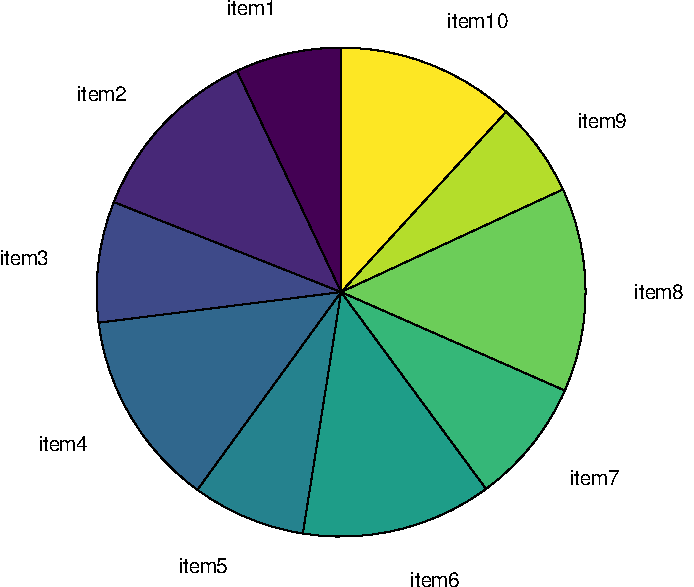
\includegraphics[width=0.6\textwidth,height=0.6\textheight,keepaspectratio]{figures/piex.pdf}
 \caption{Gráfico pizza gerado pelo código na lista \ref{lst-pie-ex}. Qual item é maior? e menor?}
 \label{fig-piex}
\end{figure}


\begin{figure}[h]
 \centering
  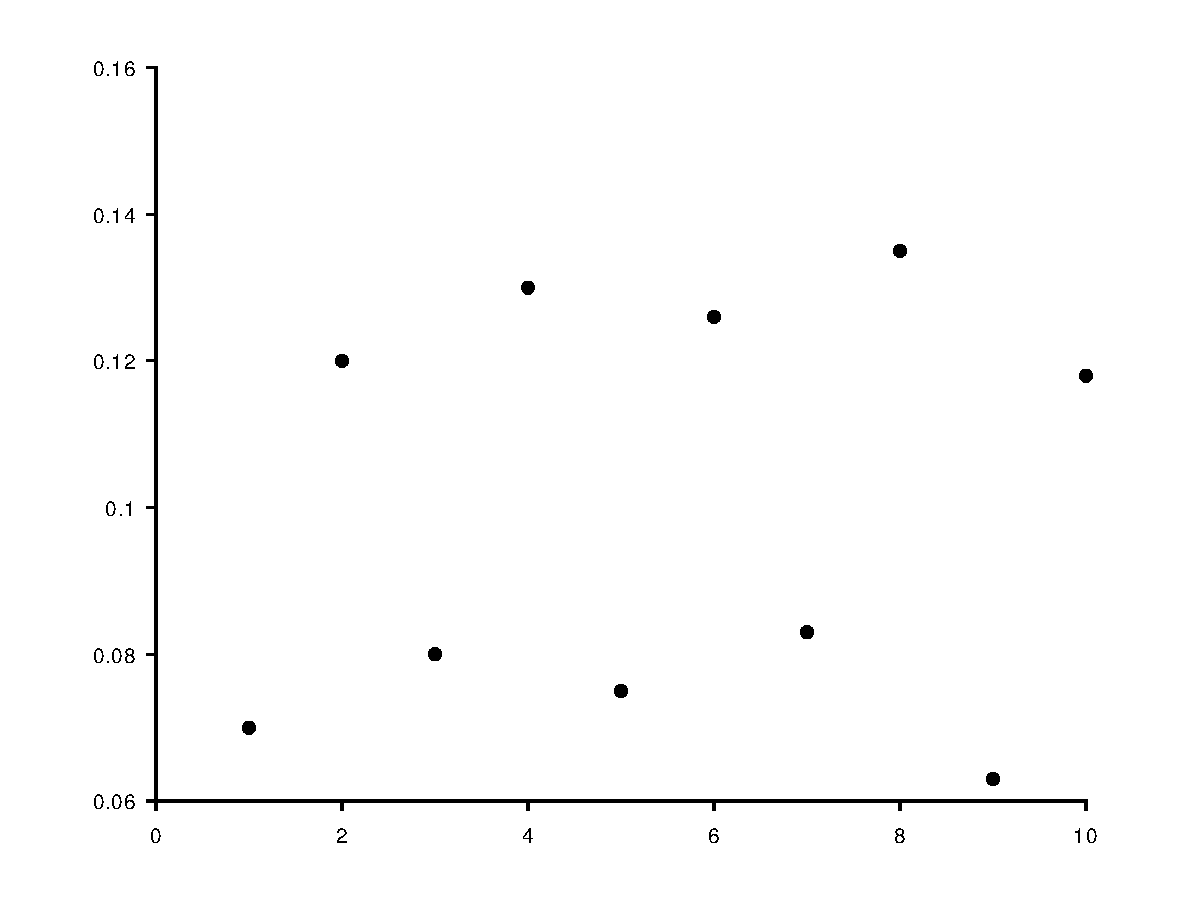
\includegraphics[width=0.8\textwidth,height=0.7\textheight,keepaspectratio]{figures/piex-dots.pdf}
 \caption{Gráfico de pontos gerado pelo código na lista \ref{lst-pie-ex}. É possível distinguir dois grupos.}
 \label{fig-piex2}
\end{figure}

\begin{figure}[h]
 \centering
  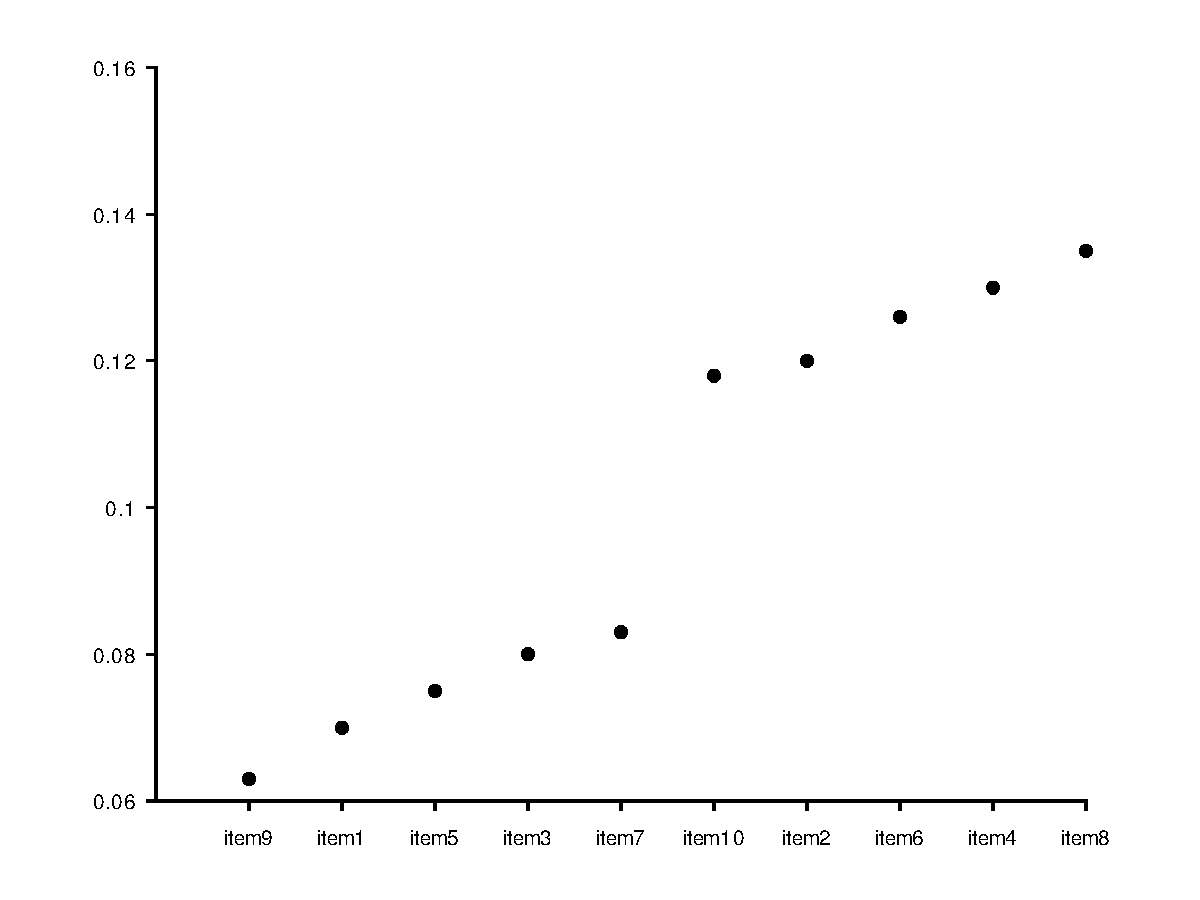
\includegraphics[width=0.8\textwidth,height=0.65\textheight,keepaspectratio]{figures/piex-dots-order.pdf}
 \caption{Gráfico de pontos gerado pelo código na lista \ref{lst-pie-ex}. É possível distinguir dois grupos e verificar a ordem de valores dos itens.}
 \label{fig-piex3}
\end{figure}

\begin{quote}
"Pie charts have severe perceptual problems. Experiments in graphical perception have shown
that compared with dot charts, they convey information far
less reliably. But if you want to display some data, and perceiving the information is not so important, then a pie chart
is fine." \cite{becker1996}
\end{quote}

\begin{quote}
"dumb pie chart; the only worse design than a pie chart is several of them,
for then the viewer is asked to compare quantities located in
spatial disarray both within and between pies. ... Given their
low data-density and failure to order numbers along a visual
dimension, pie charts should never be used." \cite{tufte_visual_1999}
\end{quote}

\framebreak

\begin{figure}[h]
 \centering
  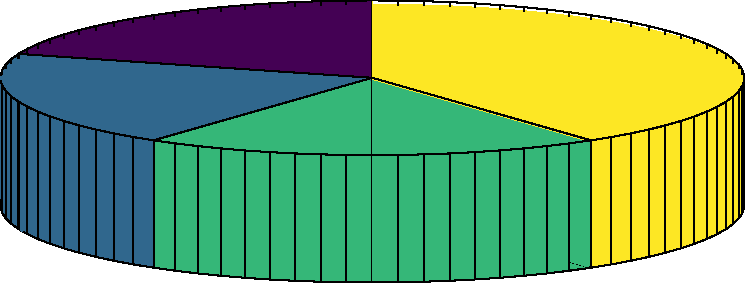
\includegraphics[width=0.7\textwidth,height=0.5\textheight,keepaspectratio]{figures/pie3d.pdf}
 \caption{Nada é tão ruim que não possa piorar.}
 \label{fig-pie3d}
\end{figure}

\framebreak

\begin{figure}[h]
 \centering
  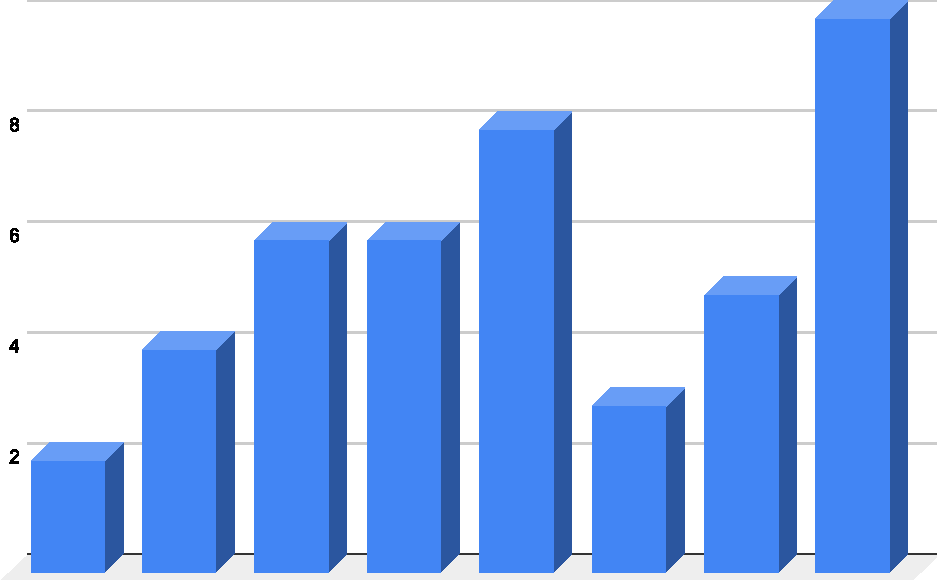
\includegraphics[width=0.7\textwidth,height=0.5\textheight,keepaspectratio]{figures/3dbars.pdf}
 \caption{Evite gráficos com 3D desnecessários.}
 \label{fig-3dbars}
\end{figure}

\end{frame}


\begin{frame}[allowframebreaks]
\frametitle{Playfair's Balance-of-Trade}

\begin{figure}[h]
 \centering
  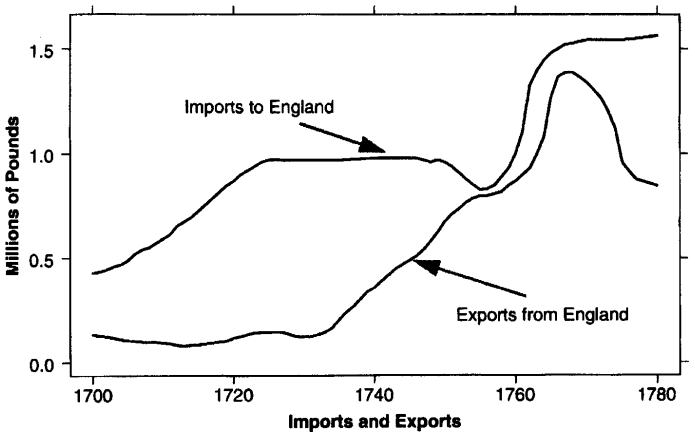
\includegraphics[width=0.7\textwidth,height=0.6\textheight,keepaspectratio]{figures/imports-exports.png}
 \caption{Balanço de comércio.}
 \label{fig-importex1}
\end{figure}

\framebreak

\begin{figure}[h]
 \centering
  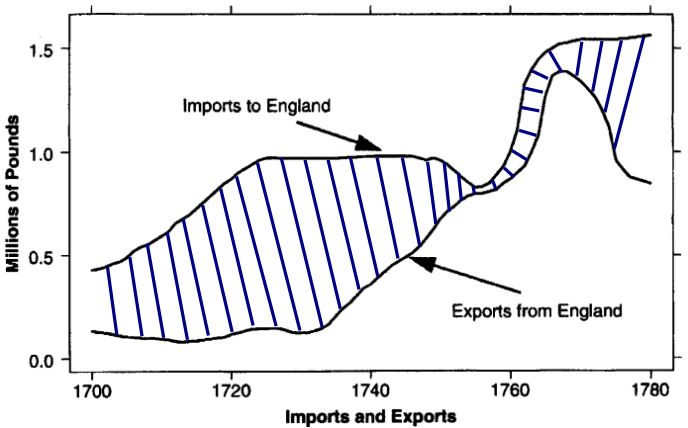
\includegraphics[width=0.7\textwidth,height=0.6\textheight,keepaspectratio]{figures/imports-exports_a.png}
 \caption{Balanço de comércio.}
 \label{fig-importex1a}
\end{figure}

\framebreak

\begin{figure}[h]
 \centering
  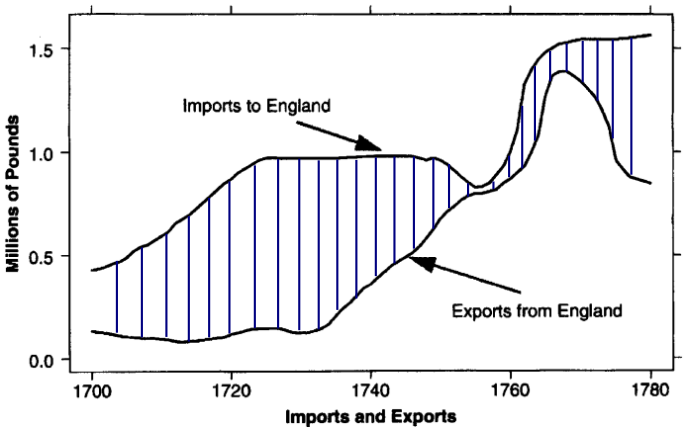
\includegraphics[width=0.7\textwidth,height=0.6\textheight,keepaspectratio]{figures/imports-exports_b.png}
 \caption{Balanço de comércio.}
 \label{fig-importex1b}
\end{figure}

\framebreak

\begin{figure}[h]
 \centering
  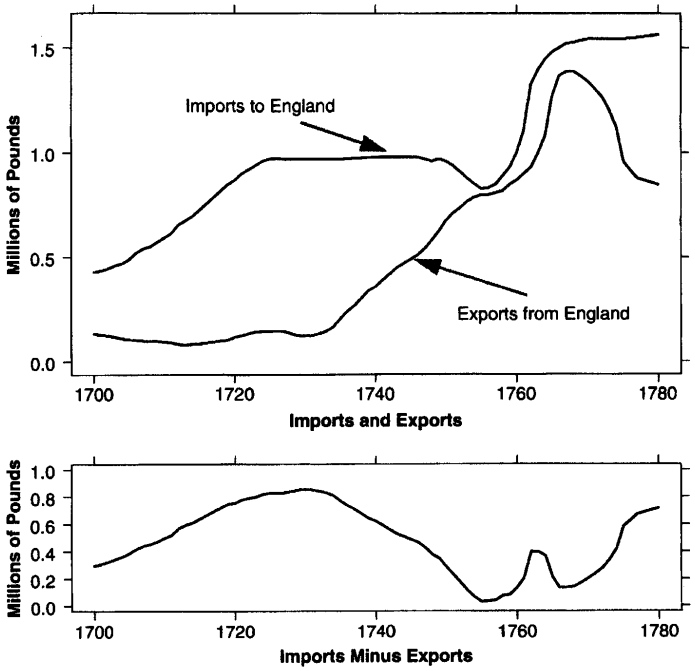
\includegraphics[width=0.7\textwidth,height=0.9\textheight,keepaspectratio]{figures/imports-exports2.png}
 \caption{Balanço de comércio.}
 \label{fig-importex2}
\end{figure}

\end{frame}




\begin{frame}[allowframebreaks,fragile]
\frametitle{Limitações de alguns gráficos}

\begin{lstlisting}[language=Octave, label=lst-y1y2, caption={Onde as curvas $y_1$ e $y_2$ estão mais próximas e mais distantes?}, postbreak=\mbox{$\hookrightarrow$\space}, basicstyle=\fontsize{8}{10}\selectfont\ttfamily]
x = [0.5:0.125:3];
y1 = 1./x.^2; y2 = y1 + 0.6;
plot(x,y1,'-',x,y2,'--'); legend('y_1','y_2');
print -dsvg curvesy1y2.svg
\end{lstlisting}

\begin{figure}[h]
 \centering
  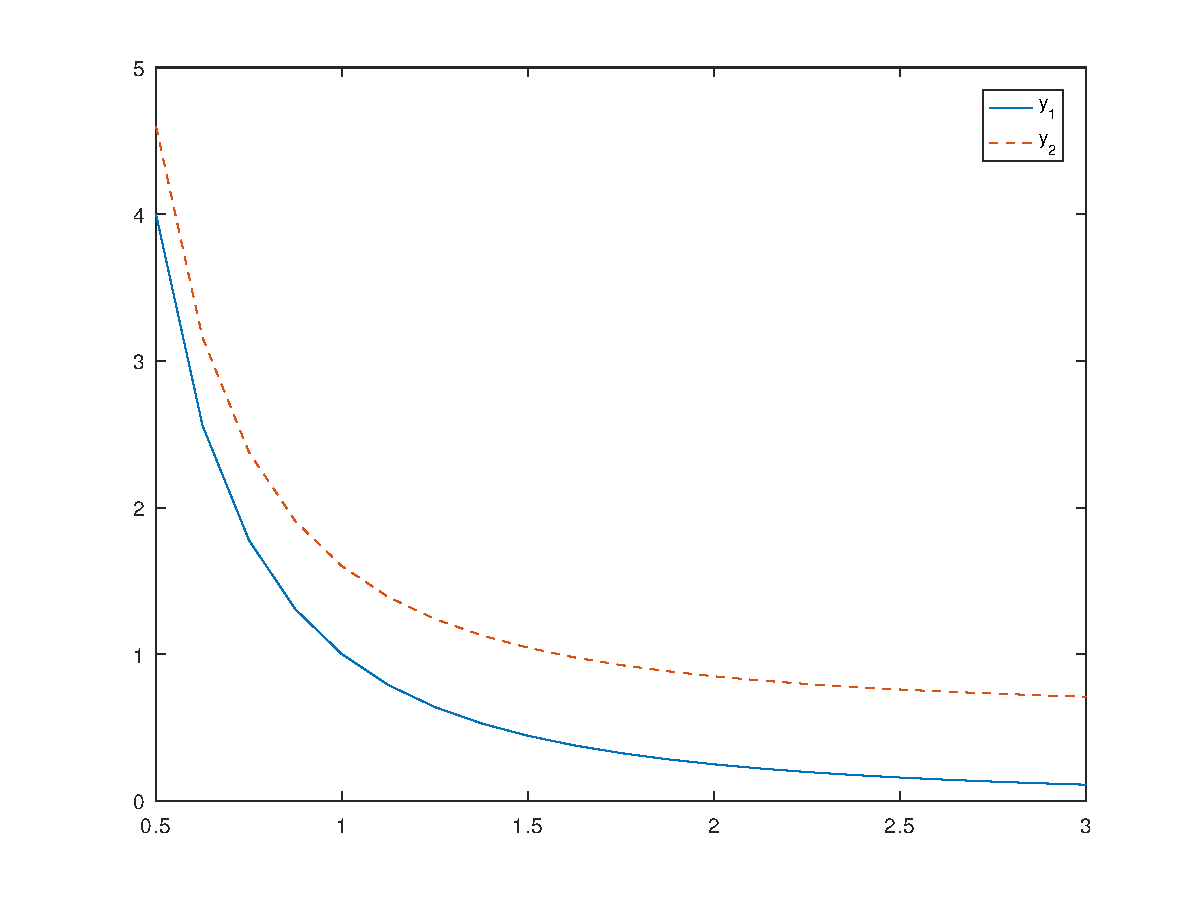
\includegraphics[width=0.7\textwidth,height=0.9\textheight,keepaspectratio]{figures/curvesy1y2.pdf}
 \caption{Diferença entre as curvas.}
 \label{fig-curvesy1y2}
\end{figure}

\end{frame}


\begin{frame}[allowframebreaks,fragile]
\frametitle{Limitações de alguns gráficos}
\begin{lstlisting}[language=Octave, label=lst-y1y2, caption={Onde as curvas $y_1$ e $y_2$ estão mais próximas e mais distantes?}, postbreak=\mbox{$\hookrightarrow$\space}, basicstyle=\fontsize{8}{10}\selectfont\ttfamily]
system('wget https://gist.githubusercontent.com/curran/13d30e855d48cdd6f22acdf0afe27286/raw/0635f14817ec634833bb904a47594cc2f5f9dbf8/worldcities_clean.csv -O /tmp/worldcities.csv')
X = csvread ('/tmp/worldcities.csv');
top100 = X(2:104,5);
id=find(top100==0);
top100(id)=[];
figure; hold on; for i=1:10:100, drawCircle(i-1,top100(i)/top100(end),top100(i)/top100(end)); end; plot([0:99],top100./top100(end),'k-'); hold off; daspect([1 1 1]);
\end{lstlisting}

\begin{figure}[h]
 \centering
  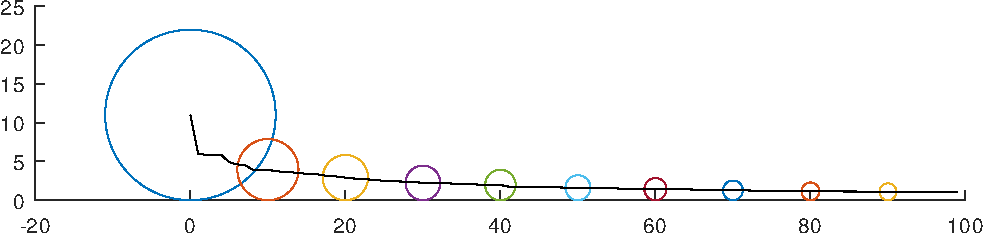
\includegraphics[width=\textwidth,height=0.5\textheight,keepaspectratio]{figures/citiespop.pdf}
 \caption{População das cidades.}
 \label{fig-citiespop}
\end{figure}

\end{frame}


\begin{frame}[allowframebreaks,fragile]
\frametitle{Limitações de alguns gráficos}
\begin{lstlisting}[language=Octave, label=lst-scatters, caption={Gráfico de espalhamento com 3 grupos.}, postbreak=\mbox{$\hookrightarrow$\space}, basicstyle=\fontsize{8}{10}\selectfont\ttfamily]
X1=rand(20,2)+0.25; X2=0.8*rand(20,2)+0.5; X3=0.6*rand(20,2)+0.75;
figure; hold on; scatter(X1(:,1),X1(:,2),40,[0 0 0],'o','filled'); scatter(X2(:,1),X2(:,2),40,[0 0 0],'s','filled'); scatter(X3(:,1),X3(:,2),40,[0 0 0],'v','filled'); hold off;
print -dsvg scatterplot1.svg
figure; hold on; scatter(X1(:,1),X1(:,2),40,[0 0 0],'o','filled'); scatter(X2(:,1),X2(:,2),40,[0.3 0.3 0.3],'s','filled'); scatter(X3(:,1),X3(:,2),40,[0.6 0.6 0.6],'v','filled'); hold off;
print -dsvg scatterplot2.svg
\end{lstlisting}

\framebreak 

\begin{figure}[h]
 \centering
  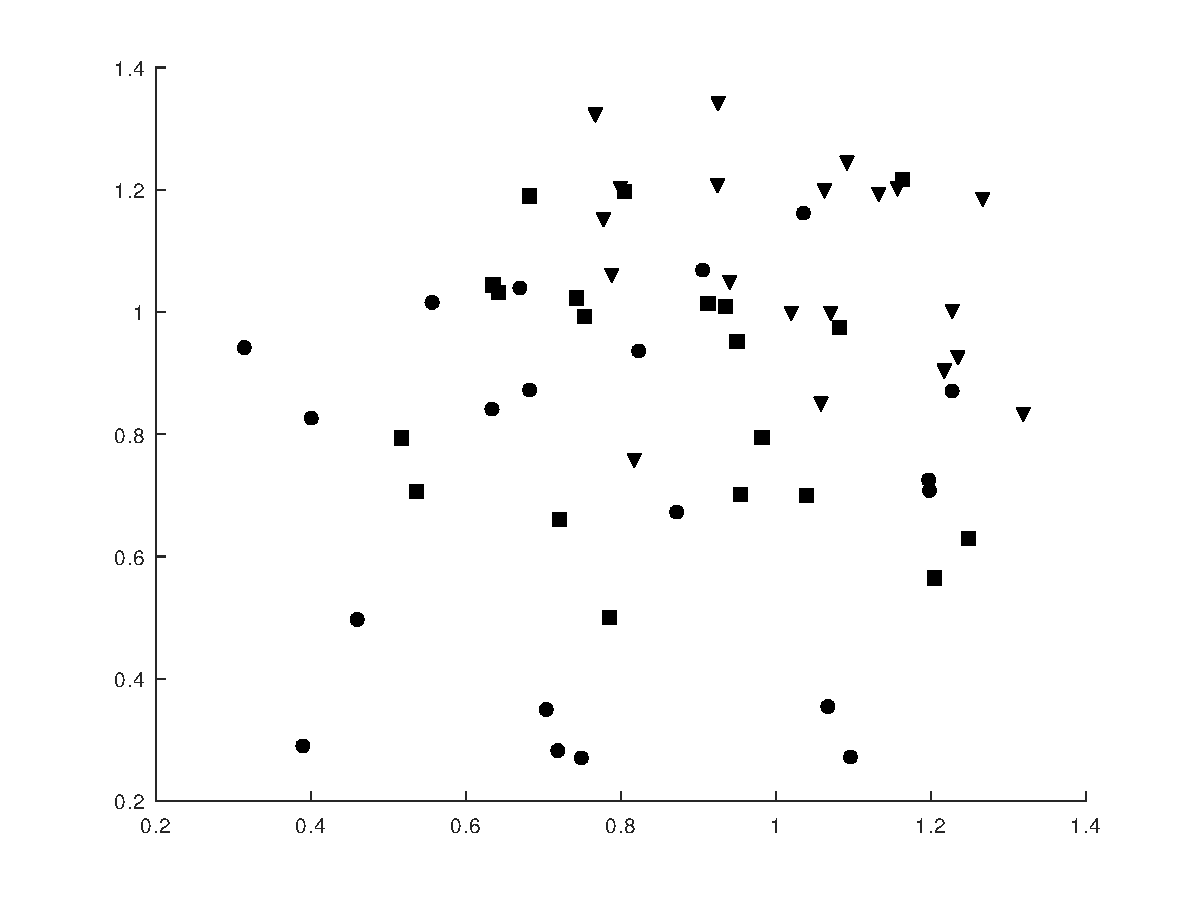
\includegraphics[width=0.7\textwidth,height=0.7\textheight,keepaspectratio]{figures/scatterplot1.pdf}
 \caption{Gráfico de espalhamento utilizando tipo de elemento para distinguir os grupos.}
 \label{fig-scatterplot1}
\end{figure}


\framebreak

\begin{figure}[h]
 \centering
  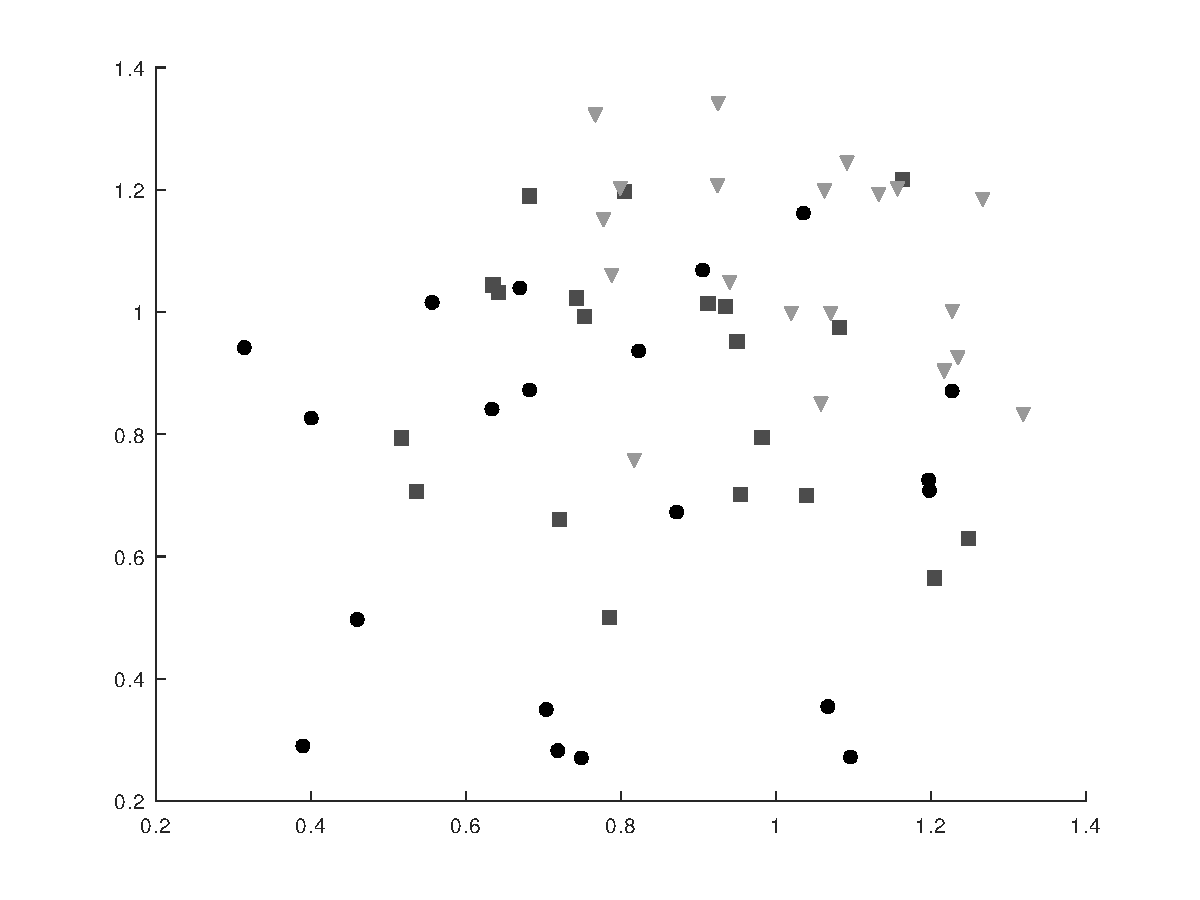
\includegraphics[width=0.7\textwidth,height=0.7\textheight,keepaspectratio]{figures/scatterplot2.pdf}
 \caption{Gráfico de espalhamento utilizando também a cor para distinguir os grupos.}
 \label{fig-scatterplot2}
\end{figure}

\end{frame}


\begin{frame}[allowframebreaks,fragile]
\frametitle{Limitações de alguns gráficos}
\begin{lstlisting}[language=Octave, label=lst-scatters, caption={Gráfico de espalhamento com 3 grupos.}, postbreak=\mbox{$\hookrightarrow$\space}, basicstyle=\fontsize{8}{10}\selectfont\ttfamily]
x = [4 11 22 29 38 42 49 7 13 22 31 39 42 49 7 14 23 32 40 43 55 9 15 27 33 40 45 58 10 15 27 33 40 47 66 10 20 28 35 40 48 72 11 21 28 38 42 48 73];
plot(x,0,'ko'); ylim ([-5 5]);
set(gca,'Visible','off')
axes('Position',get(gca,'Position'),'XAxisLocation','bottom','YAxisLocation','left', 'Color','none','XTickLabel',get(gca,'XTickLabel'),'YTickLabel',get(gca,'YTickLabel'),'XColor','k','YColor','k','LineWidth',1,'TickDir','out');
print -dsvg strip1.svg

plot(x,0.125*randn(1,length(x)),'ko'); ylim ([-5 5]);
set(gca,'Visible','off')
axes('Position',get(gca,'Position'),'XAxisLocation','bottom','YAxisLocation','left', 'Color','none','XTickLabel',get(gca,'XTickLabel'),'YTickLabel',get(gca,'YTickLabel'),'XColor','k','YColor','k','LineWidth',1,'TickDir','out');
print -dsvg strip2.svg
\end{lstlisting}

\framebreak

\begin{figure}[h]
 \centering
  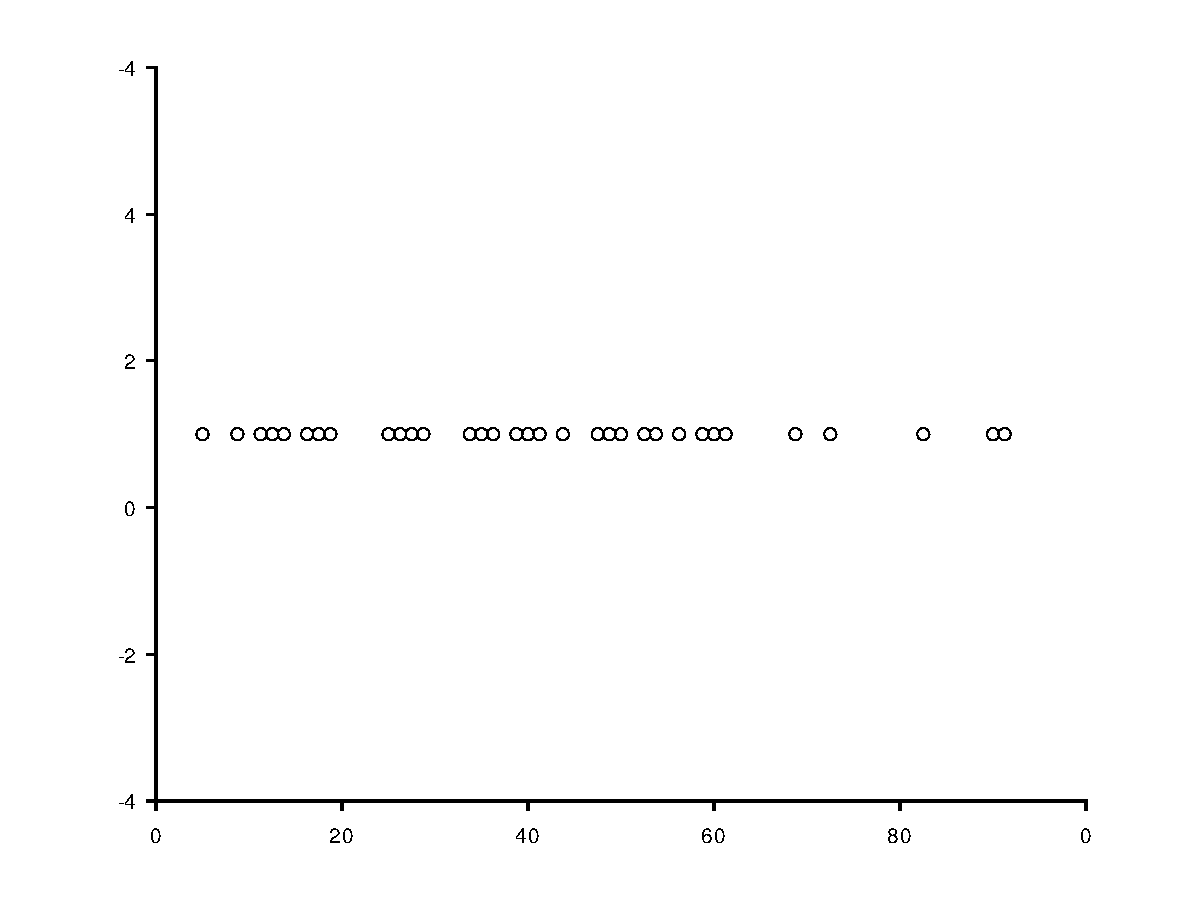
\includegraphics[width=0.7\textwidth,height=0.7\textheight,keepaspectratio]{figures/strip1.pdf}
 \caption{Strip plot.}
 \label{fig-strip1}
\end{figure}

\framebreak

\begin{figure}[h]
 \centering
  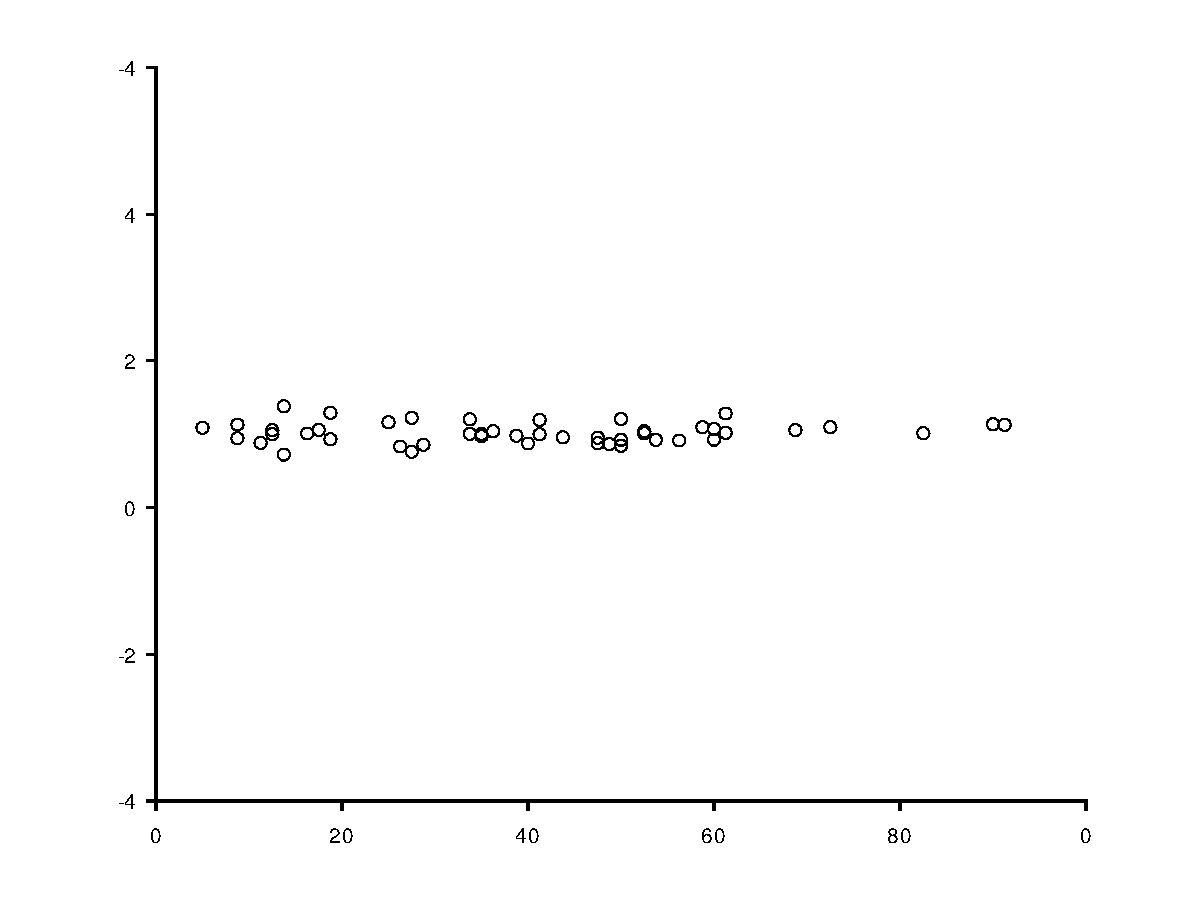
\includegraphics[width=0.7\textwidth,height=0.7\textheight,keepaspectratio]{figures/strip2.pdf}
 \caption{Strip plot com Jittering - possibilita a visualização de pontos sobrepostos.}
 \label{fig-strip2}
\end{figure}

\end{frame}





\begin{frame}[allowframebreaks]
\frametitle{Percepção de elementos gráficos}
\begin{itemize}
\item ângulo  
\item área e volume 
\item matiz de cor
\item saturação de cor
\item densidade
\item comprimento
\item posição em uma escala
\item posição ao longo de escalas não alinhadas
\item inclinação
\end{itemize}

\begin{quote}
Distance and detection also play a role in our ability to decode
information from graphs. The closer together objects are, the
easier it is to judge attributes that compare them. As distance
between objects increases, accuracy of judgment decreases. It
is certainly easier to judge the difference in lengths of two bars
if they are next to one another than if they are pages apart.
\cite{robbins_creating_2013}
\end{quote}

\end{frame}



\begin{frame}
Sugestões de leitura: 
\vspace{2ex}

\fullcite{harford_florence}
\vspace{2ex}

\fullcite{tufte_visual_1999}
\vspace{2ex}

\fullcite{tufte_beautiful_2006}
\vspace{2ex}

\fullcite{knaflic_storytelling_2015}
\vspace{2ex}

\fullcite{robbins_creating_2013}
\end{frame}


\begin{frame}
\frametitle{Figuras}
Tipos de figuras:
\begin{itemize}
\item vetoriais (.pdf, .eps, .svg, .dwg)
\item rasterizadas (.jpg, .png,. gif)
\end{itemize}
\end{frame}


\begin{frame}
\begin{figure}[h]
 \centering
 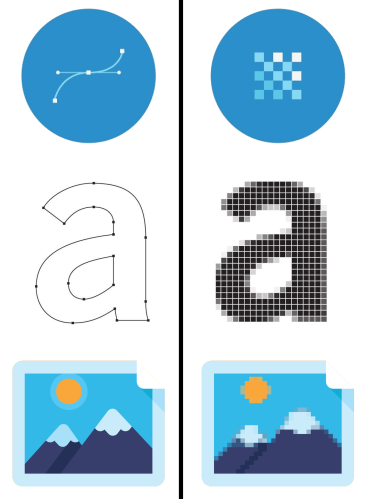
\includegraphics[width=0.45\textwidth,height=0.8\textheight,keepaspectratio]{figures/vector-raster.png}
 \caption{Imagem vetorial vs imagem rasterizada.}
 \label{fig-imgvr}
\end{figure}
\end{frame}

\begin{frame}[fragile]
\frametitle{Inserindo uma imagem em \LaTeX{}}
\begin{lstlisting}[language=tex, label=lst-figure, caption={Código para inserir uma figura em \LaTeX{}}, postbreak=\mbox{$\hookrightarrow$\space}, basicstyle=\fontsize{8}{10}\selectfont\ttfamily]
\begin{figure}[htbp]
 \centering
 \includegraphics[width=0.5\textwidth]{example-image-a}
 \caption{Legenda da figura.}
 \label{fig-img-a}
\end{figure}
\end{lstlisting}
\end{frame}



\begin{frame}
\frametitle{Tikz}
\begin{figure}[h]
\centering
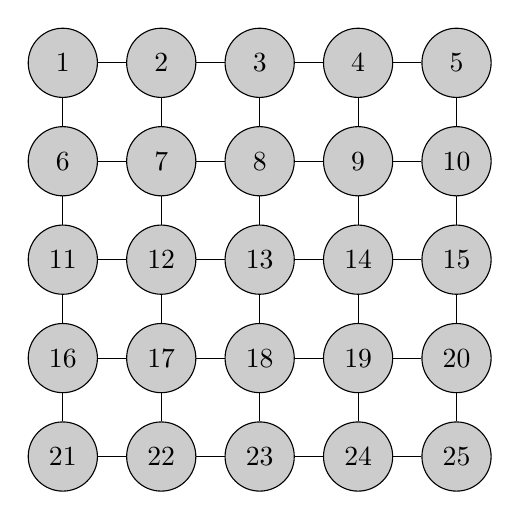
\begin{tikzpicture}[darkstyle/.style={circle,draw,fill=gray!40,minimum size=25}]
  \foreach \x in {0,...,4}
    \foreach \y in {0,...,4} 
       {\pgfmathtruncatemacro{\label}{\x - 5 *  \y +21}
       \node [darkstyle]  (\x\y) at (1.25*\x,1.25*\y) {\label};} 

  \foreach \x in {0,...,4}
    \foreach \y [count=\yi] in {0,...,3}  
      \draw (\x\y)--(\x\yi) (\y\x)--(\yi\x) ;
\end{tikzpicture}
\caption{Exemplo de utilização do Tikz.}
 \label{fig-tikz}
\end{figure}
\end{frame}


\begin{frame}[fragile]
\frametitle{Código exemplo Tikz}
\begin{lstlisting}[language=tex, label=lst-tikz, caption={Código utilizado para criar o exemplo em tikz.}, postbreak=\mbox{$\hookrightarrow$\space}, basicstyle=\fontsize{8}{10}\selectfont\ttfamily]
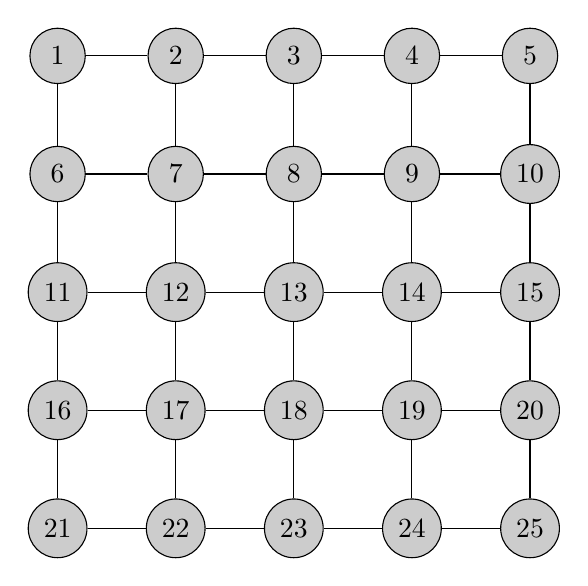
\begin{tikzpicture}[darkstyle/.style={circle,draw,fill=gray!40,minimum size=20}]
 \foreach \x in {0,...,4}
   \foreach \y in {0,...,4} 
      {\pgfmathtruncatemacro{\label}{\x - 5 *  \y +21}
      \node [darkstyle]  (\x\y) at (1.5*\x,1.5*\y) {\label};} 

 \foreach \x in {0,...,4}
   \foreach \y [count=\yi] in {0,...,3}  
     \draw (\x\y)--(\x\yi) (\y\x)--(\yi\x) ;
\end{tikzpicture}
\end{lstlisting}
\end{frame}


\subsection{ggplot}
\begin{frame}
\frametitle{ggplot2}
\texttt{ggplot2} é um pacote de visualização de dados para R.

\vspace{3ex}
O \texttt{ggplot2} fornece um esquema de visualização de dados que se
utiliza de camadas de conteúdo semântico. Os dados devem ser dispostos em \emph{dataframes} 
ao invés de vetores individuais.

\end{frame}

\begin{frame}[fragile,allowframebreaks]
\frametitle{ggplot2 - wine quality data set}
\centering

\lstinputlisting[language=R, label=lst-ggplotwine-1, firstline=1, lastline=6, postbreak=\mbox{$\hookrightarrow$\space}, basicstyle=\fontsize{8}{10}\selectfont\ttfamily]{examples/ggplot-wine.r}

\framebreak
\lstinputlisting[language=R, label=lst-ggplotwine-2, firstline=7, lastline=28, postbreak=\mbox{$\hookrightarrow$\space}, basicstyle=\fontsize{8}{10}\selectfont\ttfamily]{examples/ggplot-wine.r} 

\framebreak
\lstinputlisting[language=R, label=lst-ggplotwine-3, firstline=29, lastline=34, postbreak=\mbox{$\hookrightarrow$\space}, basicstyle=\fontsize{8}{10}\selectfont\ttfamily]{examples/ggplot-wine.r} 

\framebreak
\lstinputlisting[language=R, label=lst-ggplotwine-4, firstline=36, lastline=38, postbreak=\mbox{$\hookrightarrow$\space}, basicstyle=\fontsize{8}{10}\selectfont\ttfamily]{examples/ggplot-wine.r} 
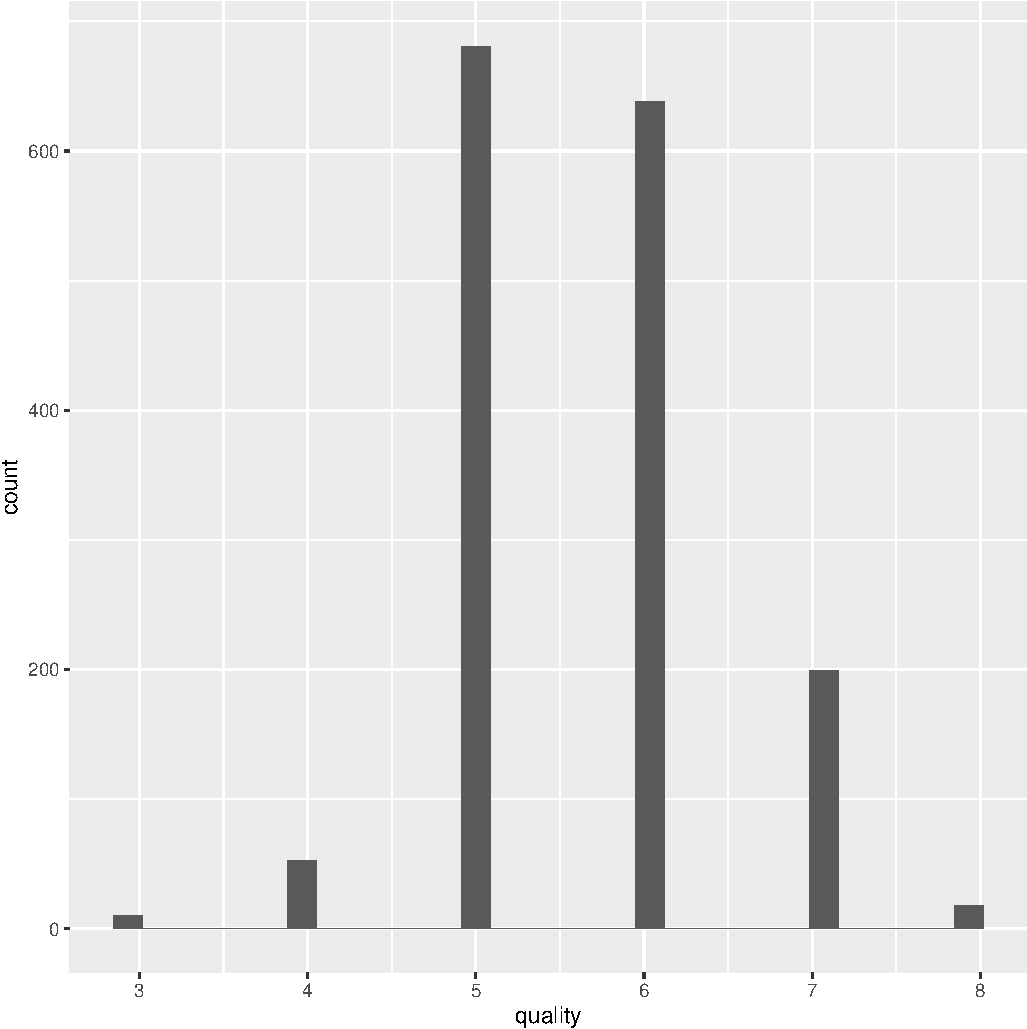
\includegraphics[width=0.8\textwidth,height=0.7\textheight,keepaspectratio]{examples/ex-ggplot-01-crop.pdf}

\framebreak
\lstinputlisting[language=R, label=lst-ggplotwine-5, firstline=39, lastline=40, postbreak=\mbox{$\hookrightarrow$\space}, basicstyle=\fontsize{8}{10}\selectfont\ttfamily]{examples/ggplot-wine.r} 
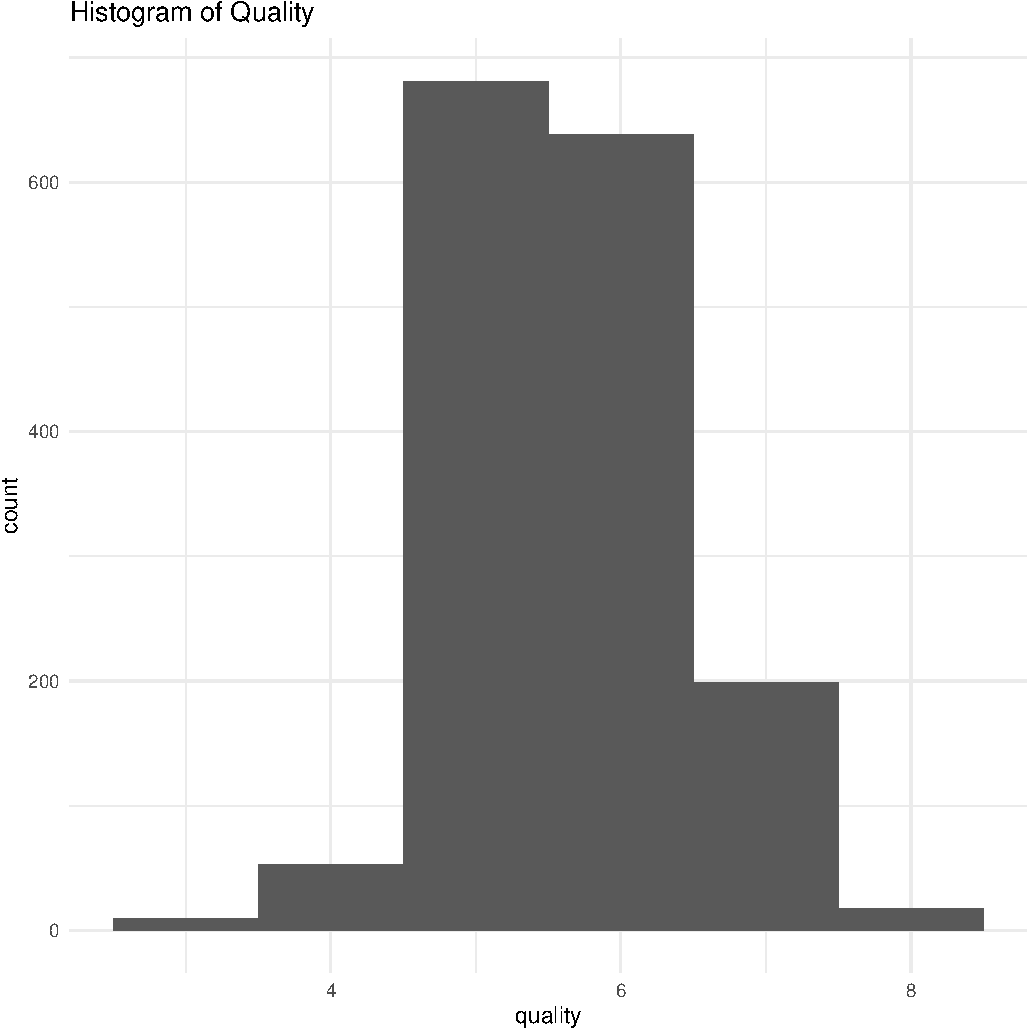
\includegraphics[width=0.8\textwidth,height=0.7\textheight,keepaspectratio]{examples/ex-ggplot-02-crop.pdf}

\framebreak
\lstinputlisting[language=R, label=lst-ggplotwine-6, firstline=41, lastline=42, postbreak=\mbox{$\hookrightarrow$\space}, basicstyle=\fontsize{8}{10}\selectfont\ttfamily]{examples/ggplot-wine.r} 
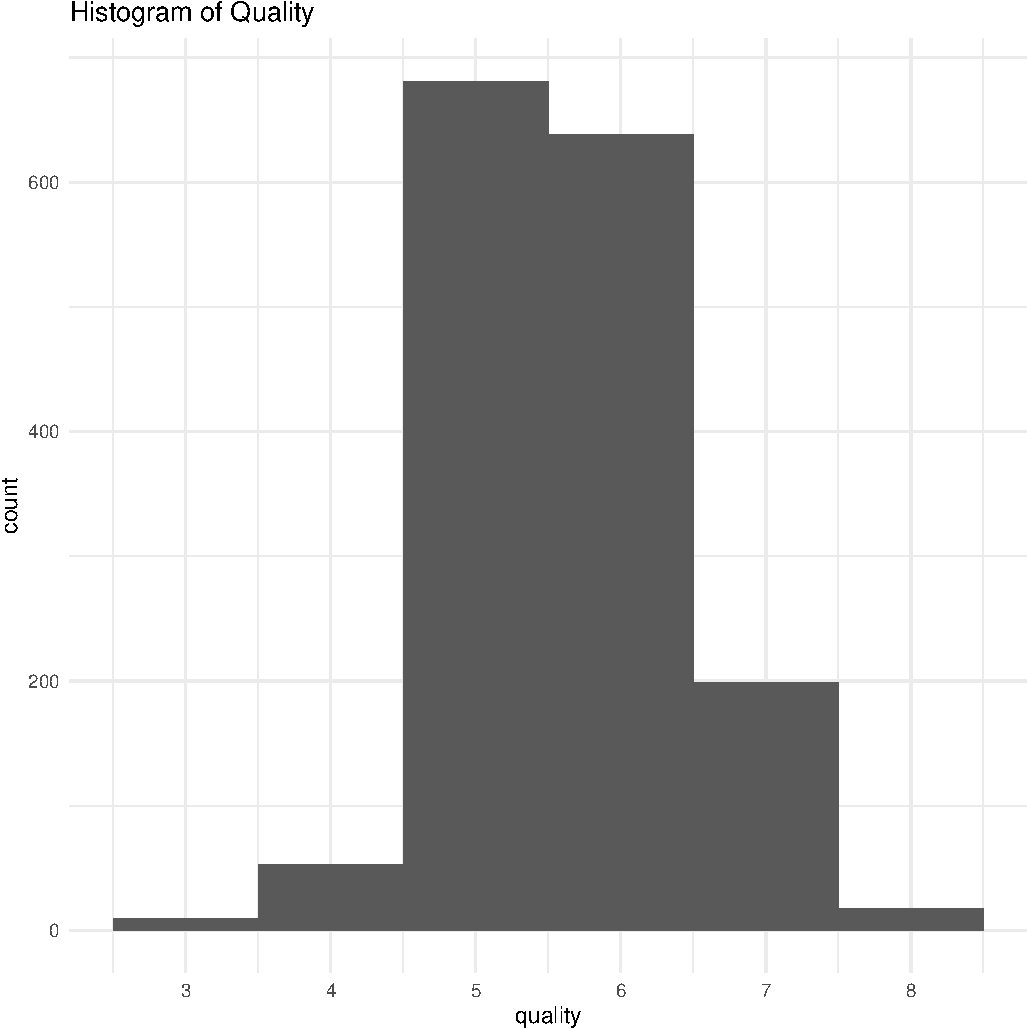
\includegraphics[width=0.8\textwidth,height=0.7\textheight,keepaspectratio]{examples/ex-ggplot-03-crop.pdf}

\framebreak
\lstinputlisting[language=R, label=lst-ggplotwine-7, firstline=43, lastline=44, postbreak=\mbox{$\hookrightarrow$\space}, basicstyle=\fontsize{8}{10}\selectfont\ttfamily]{examples/ggplot-wine.r} 

\includegraphics[width=0.8\textwidth,height=0.7\textheight,keepaspectratio]{examples/ex-ggplot-04-crop.pdf}

\framebreak
\lstinputlisting[language=R, label=lst-ggplotwine-8, firstline=45, lastline=46, postbreak=\mbox{$\hookrightarrow$\space}, basicstyle=\fontsize{8}{10}\selectfont\ttfamily]{examples/ggplot-wine.r} 
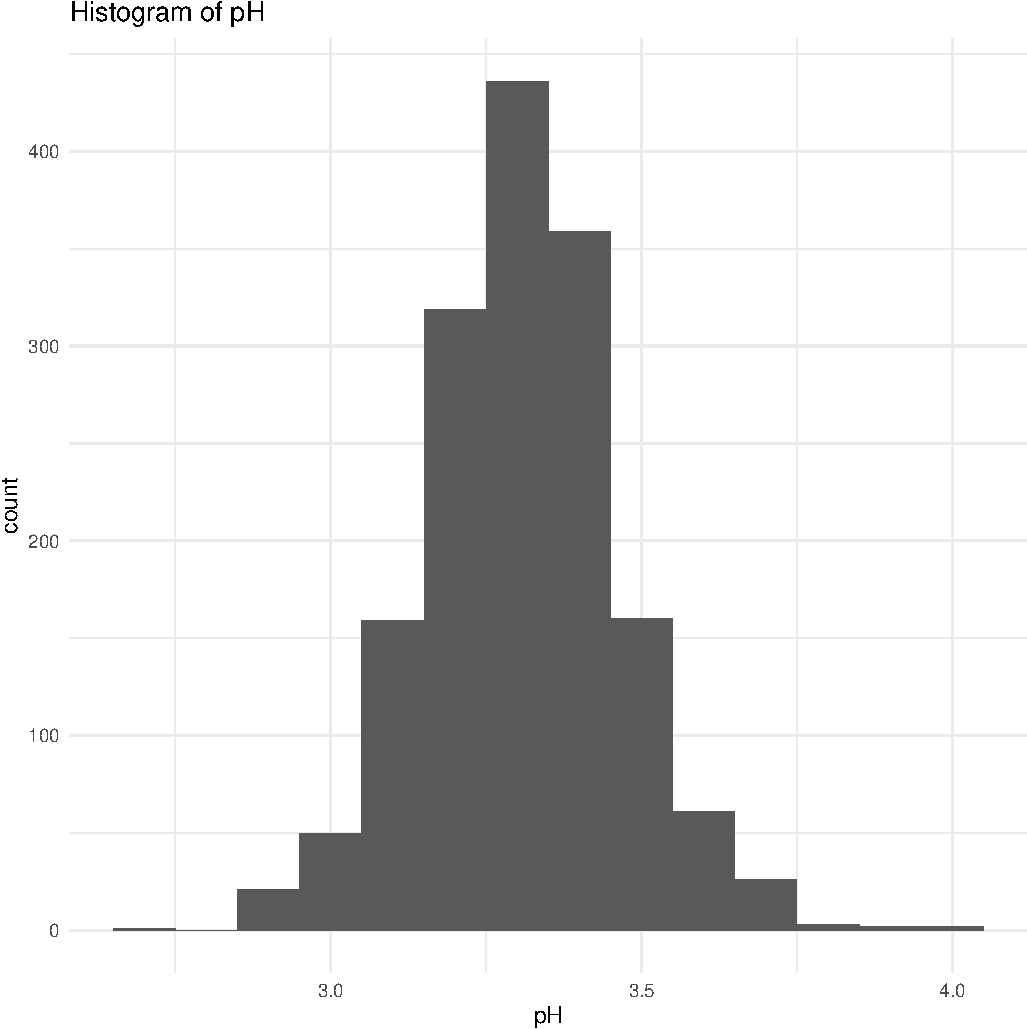
\includegraphics[width=0.8\textwidth,height=0.7\textheight,keepaspectratio]{examples/ex-ggplot-05-crop.pdf}

\framebreak
\lstinputlisting[language=R, label=lst-ggplotwine-9, firstline=47, lastline=48, postbreak=\mbox{$\hookrightarrow$\space}, basicstyle=\fontsize{8}{10}\selectfont\ttfamily]{examples/ggplot-wine.r} 
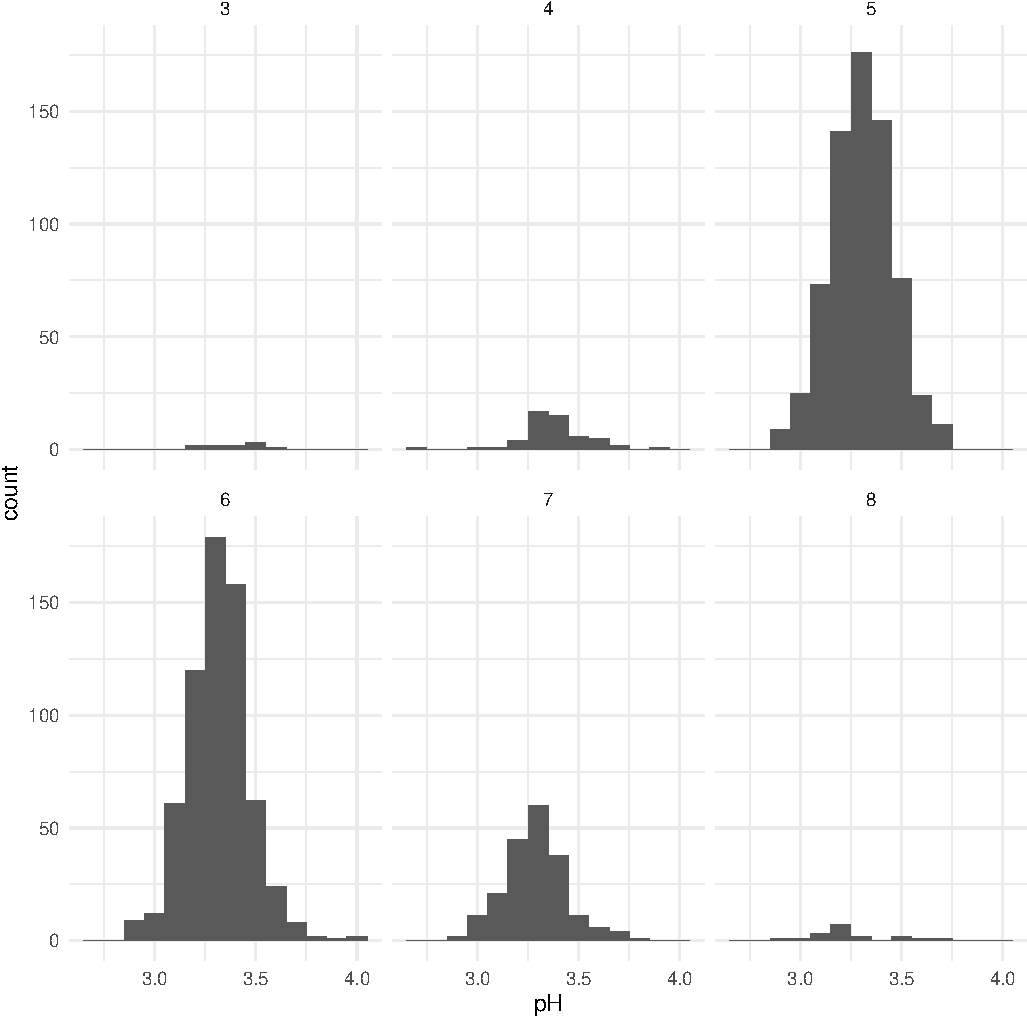
\includegraphics[width=0.8\textwidth,height=0.7\textheight,keepaspectratio]{examples/ex-ggplot-06-crop.pdf}

\framebreak
\lstinputlisting[language=R, label=lst-ggplotwine-10, firstline=49, lastline=50, postbreak=\mbox{$\hookrightarrow$\space}, basicstyle=\fontsize{8}{10}\selectfont\ttfamily]{examples/ggplot-wine.r} 
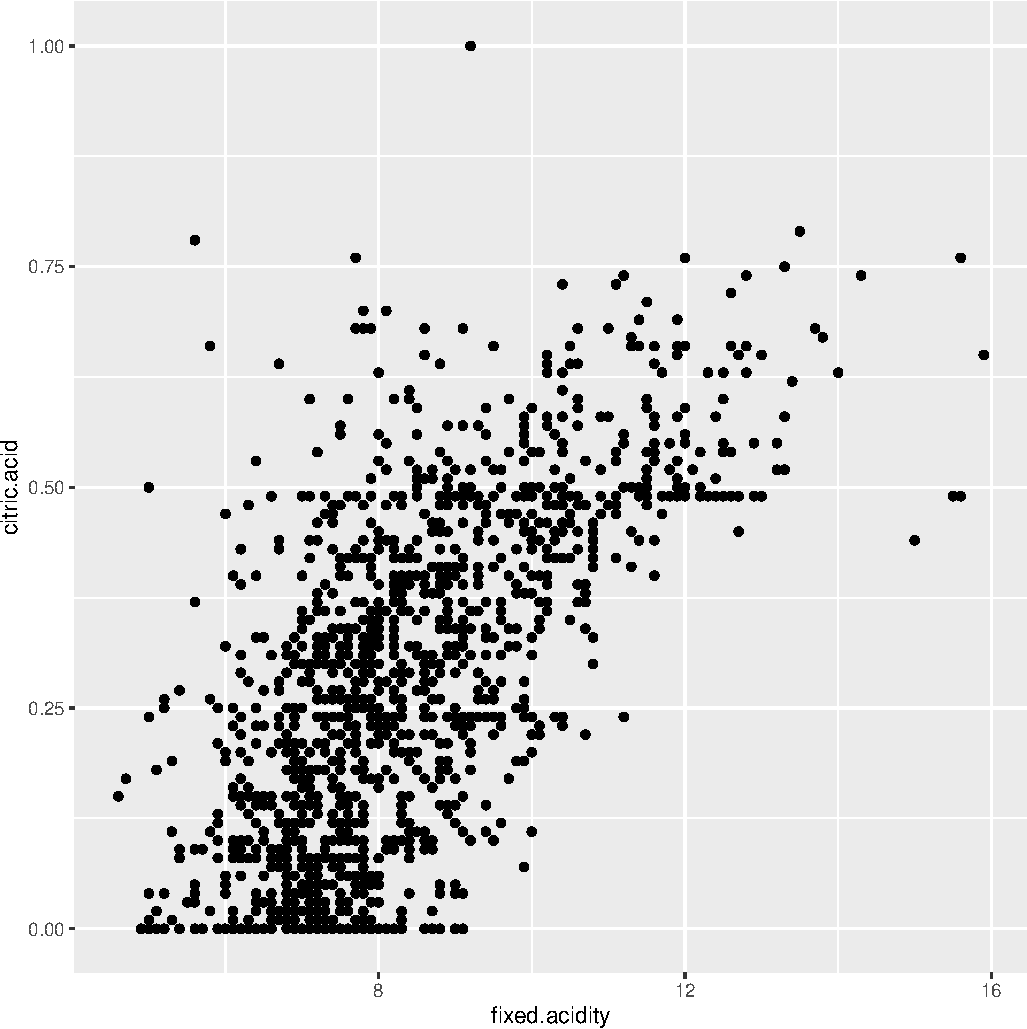
\includegraphics[width=0.8\textwidth,height=0.7\textheight,keepaspectratio]{examples/ex-ggplot-07-crop.pdf}

\framebreak
\lstinputlisting[language=R, label=lst-ggplotwine-11, firstline=51, lastline=52, postbreak=\mbox{$\hookrightarrow$\space}, basicstyle=\fontsize{8}{10}\selectfont\ttfamily]{examples/ggplot-wine.r} 
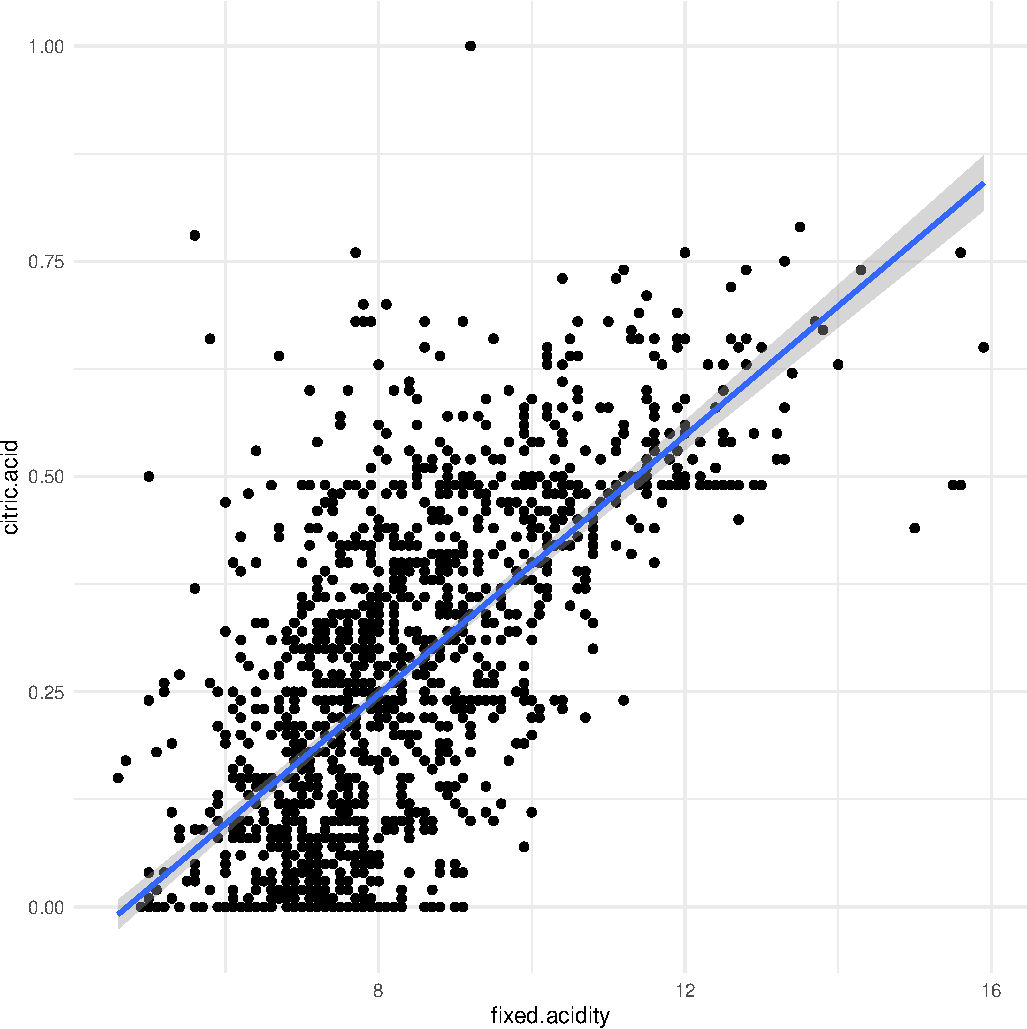
\includegraphics[width=0.8\textwidth,height=0.7\textheight,keepaspectratio]{examples/ex-ggplot-08-crop.pdf}

\framebreak
\lstinputlisting[language=R, label=lst-ggplotwine-12, firstline=53, lastline=54, postbreak=\mbox{$\hookrightarrow$\space}, basicstyle=\fontsize{8}{10}\selectfont\ttfamily]{examples/ggplot-wine.r} 
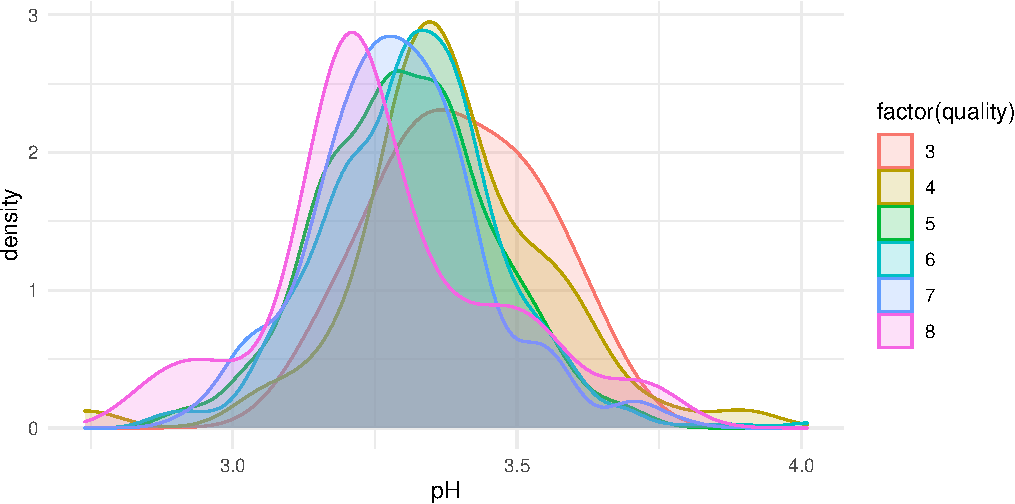
\includegraphics[width=0.8\textwidth,height=0.7\textheight,keepaspectratio]{examples/ex-ggplot-09-crop.pdf}

\framebreak
\lstinputlisting[language=R, label=lst-ggplotwine-13, firstline=55, lastline=56, postbreak=\mbox{$\hookrightarrow$\space}, basicstyle=\fontsize{8}{10}\selectfont\ttfamily]{examples/ggplot-wine.r} 
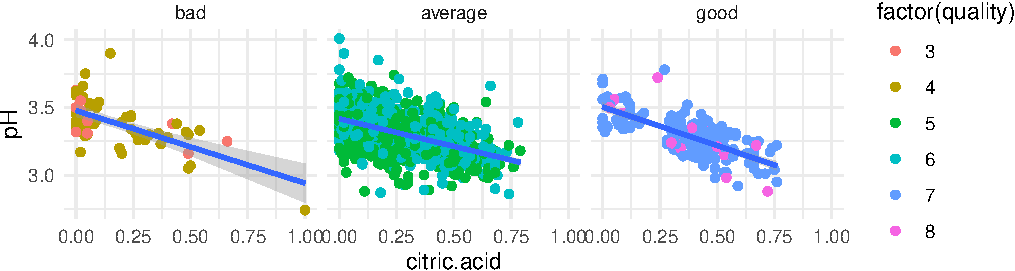
\includegraphics[width=0.8\textwidth,height=0.7\textheight,keepaspectratio]{examples/ex-ggplot-10-crop.pdf}

\framebreak
\lstinputlisting[language=R, label=lst-ggplotwine-14, firstline=57, lastline=58, postbreak=\mbox{$\hookrightarrow$\space}, basicstyle=\fontsize{8}{10}\selectfont\ttfamily]{examples/ggplot-wine.r} 
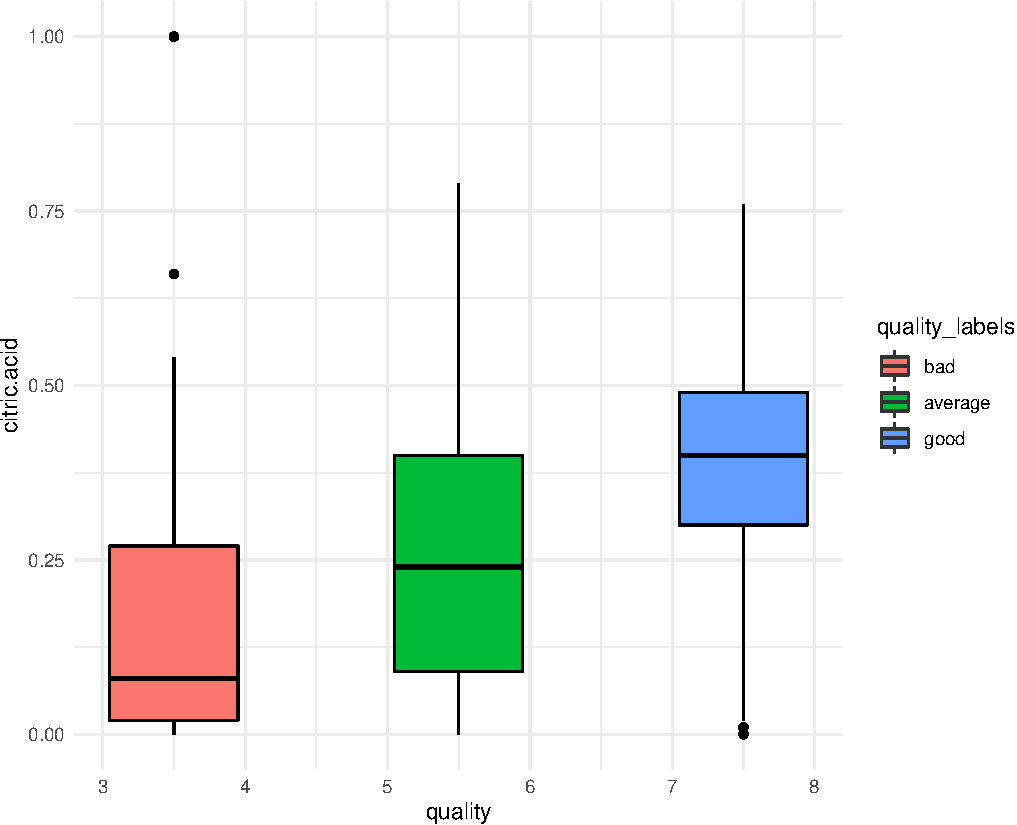
\includegraphics[width=0.8\textwidth,height=0.7\textheight,keepaspectratio]{examples/ex-ggplot-11-crop.pdf}

\end{frame}

%\multido{\i=1+1}{7}{%
%  \begin{frame}[fragile]
%  \frametitle{ggplot2 - example \i}
%  \i
%%  \centering
%%  \lstinputlisting[language=R, label=lst-ggplotwine-\i, firstline=7, lastline=28, postbreak=\mbox{$\hookrightarrow$\space}, basicstyle=\fontsize{8}{10}\selectfont\ttfamily]{examples/ggplot-wine.r}
%%  \includegraphics[width=0.8\textwidth,height=0.7\textheight,keepaspectratio]{figures/ex-ggplot-\ifnum\i<10 0\fi\i.png}
%  \end{frame}
%}


\begin{frame}
\frametitle{Gráficos de mortalidade durante a guerra da Crimeia (1853 a 1856)}
\begin{figure}[htbp]
\begin{minipage}[t]{0.49\textwidth}
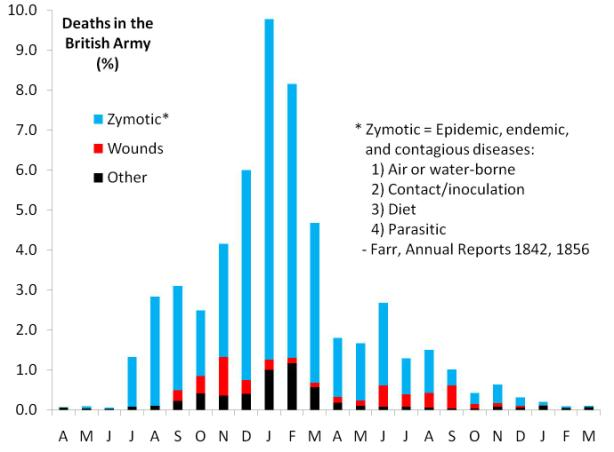
\includegraphics[width=\linewidth,height=0.8\textheight,keepaspectratio]{figures/ng_diagram2.jpg}
\subcaption{Gráfico de barras.}
\end{minipage}
\hfill
\begin{minipage}[t]{0.49\textwidth}
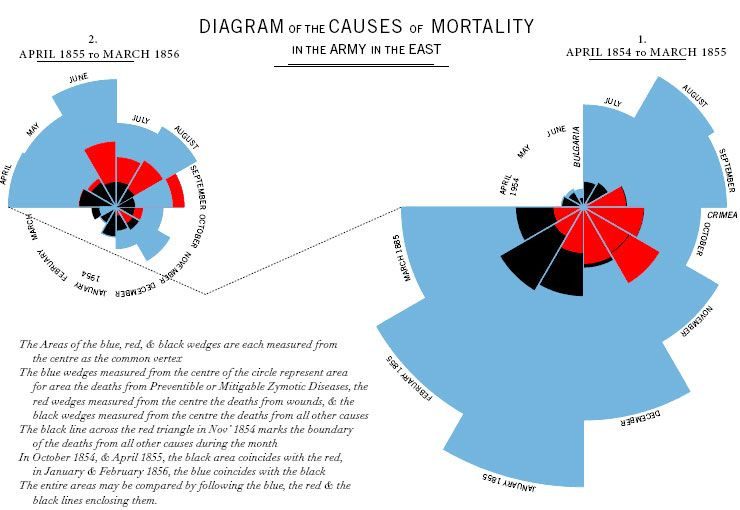
\includegraphics[width=\linewidth,height=0.8\textheight,keepaspectratio]{figures/ng_diagram1.jpg}
\subcaption{Diagrama de Florence Nightingale (\emph{coxcomb plots}).}
\end{minipage}
\caption{Comparação entre os gráficos de mortalidade utilizando os mesmos dados.}
\end{figure}
\end{frame}
% http://www.florence-nightingale-avenging-angel.co.uk/Nightingale_Hockey_Stick.pdf


\begin{frame}[allowframebreaks]
\frametitle{Florence Nightingale no R - \emph{coxcomb diagram}}
\begin{figure}[h]
 \centering
 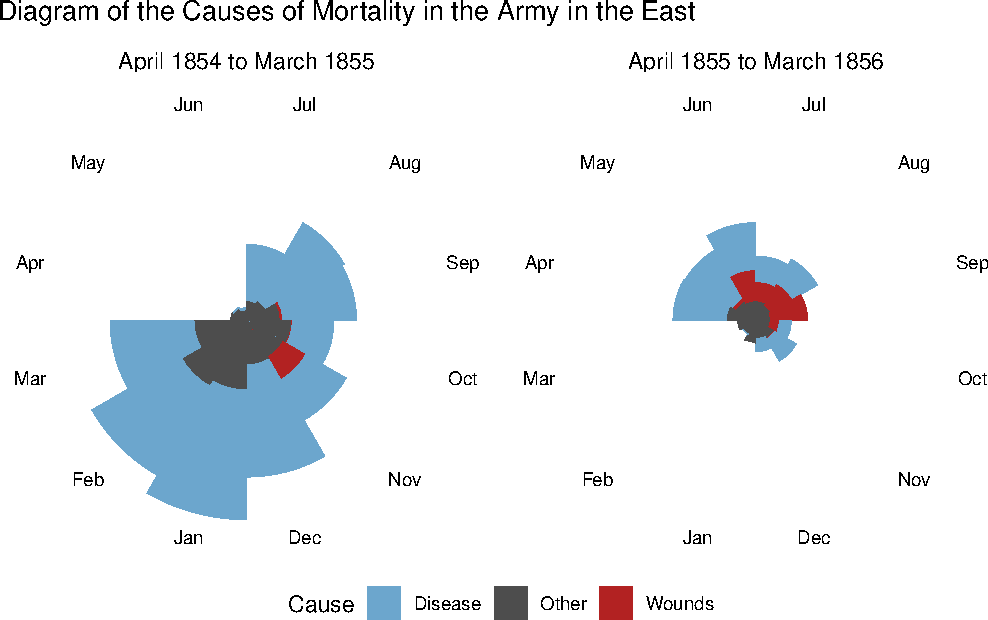
\includegraphics[width=0.8\textwidth,height=0.65\textheight,keepaspectratio]{figures/nightingale-R.pdf}
 \caption{\small Reprodução do gráfico de Florence Nightingale usando \texttt{ggplot2}. Fonte: \url{https://www.r-bloggers.com/2021/03/florence-nightingales-rose-charts-and-others-in-ggplot2/}.}
 \label{fig-nightingale-R}
\end{figure}

\framebreak

\lstinputlisting[language=R, label=lst-nightingale, postbreak=\mbox{$\hookrightarrow$\space}, basicstyle=\fontsize{8}{10}\selectfont\ttfamily]{examples/nightingale-rbloggers.R}

\end{frame}


\begin{frame}[allowframebreaks=1,fragile]
\frametitle{Mortes no Brasil 2003 a 2021}
\begin{minipage}[b]{0.47\textwidth}
\scriptsize
\begin{table}[h]
\csvstyle{mystyle}{
    tabular=lllH,
    head to column names,
    table head= {Date} & {Year} & {Month} & {Deaths} \\\midrule,
    filter={\value{csvrow}<18}
}
\csvreader[mystyle]{examples/obitos-br.csv}{}{\Date & \Year & \Month & \Deaths}
\caption{\label{tab-obitos-br}Número de óbitos no Brasil.}
\end{table}
\end{minipage}
\begin{minipage}[b]{0.47\textwidth}
\scriptsize
Dados obtidos pelo IBGE e Registro Civil:\\
\url{https://sidra.ibge.gov.br/tabela/2681#resultado} \\
\url{https://transparencia.registrocivil.org.br/registros}
\end{minipage}

\framebreak

\begin{figure}[h]
 \centering
 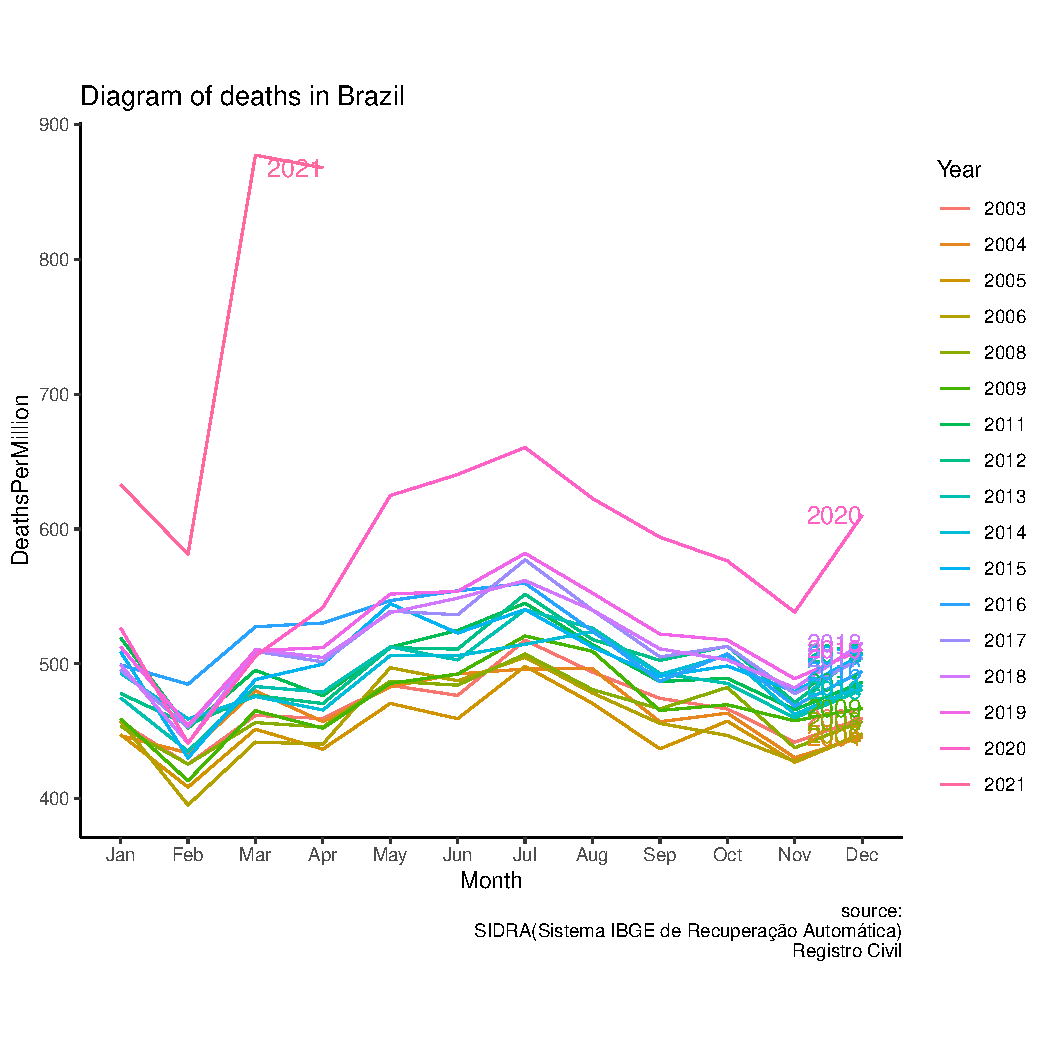
\includegraphics[width=0.8\textwidth,height=0.75\textheight,keepaspectratio]{examples/deaths-brazil-lines-per1E6.pdf}
 \caption{\small Número de óbitos no Brasil de janeiro de 2003 a abril de 2021.}
 \label{fig-deathsbr}
\end{figure}

\framebreak

\begin{figure}[h]
 \centering
 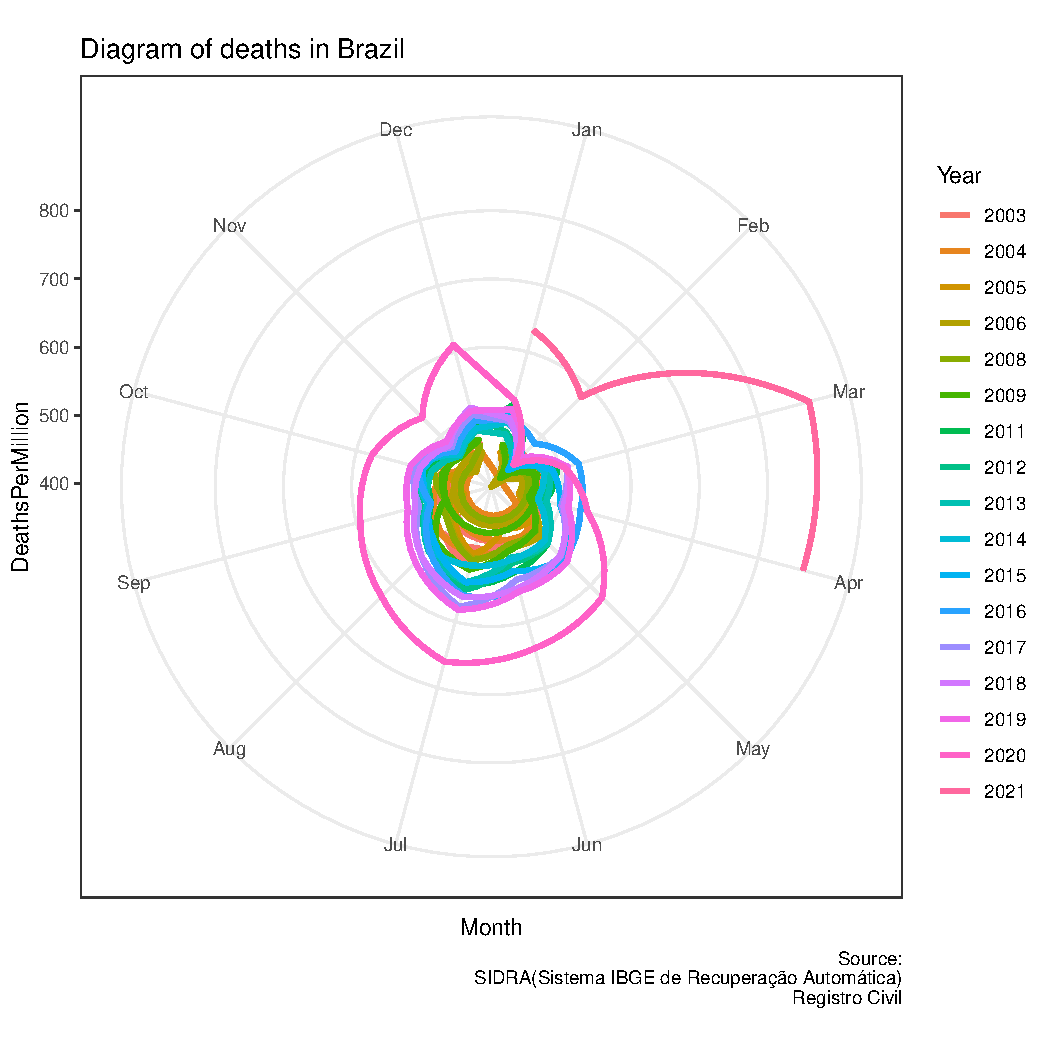
\includegraphics[width=0.8\textwidth,height=0.75\textheight,keepaspectratio]{examples/deaths-brazil-polar-per1E6.pdf}
 \caption{\small Número de óbitos no Brasil de janeiro de 2003 a abril de 2021.}
 \label{fig-deathsbr-polar}
\end{figure}

\framebreak

Carregando as bibliotecas que serão utilizadas:
\lstinputlisting[language=R, label=lst-deathsbr1, linerange={1-3}, postbreak=\mbox{$\hookrightarrow$\space}, basicstyle=\fontsize{8}{10}\selectfont\ttfamily]{examples/deaths-brazil.r}

Preparando os dados:
\lstinputlisting[language=R, label=lst-deathsbr2, linerange={5-13}, postbreak=\mbox{$\hookrightarrow$\space}, basicstyle=\fontsize{8}{10}\selectfont\ttfamily]{examples/deaths-brazil.r}

\framebreak
Gráfico linear:
\lstinputlisting[language=R, label=lst-deathsbr3, linerange={15-21}, postbreak=\mbox{$\hookrightarrow$\space}, basicstyle=\fontsize{8}{10}\selectfont\ttfamily]{examples/deaths-brazil.r}

\framebreak
Gráfico polar:
\lstinputlisting[language=R, label=lst-deathsbr4, linerange={23-31}, postbreak=\mbox{$\hookrightarrow$\space}, basicstyle=\fontsize{8}{10}\selectfont\ttfamily]{examples/deaths-brazil.r}

\end{frame}



\begin{frame}[fragile,allowframebreaks]
\frametitle{Exemplo dados condomínio}
\centering
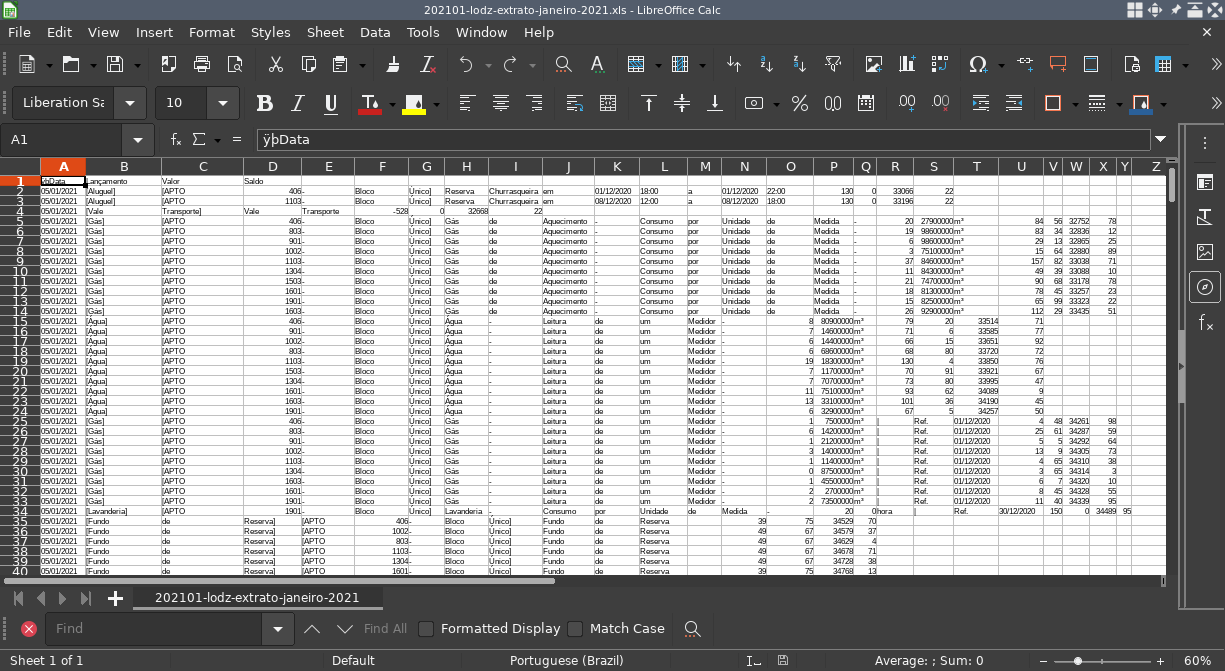
\includegraphics[width=0.8\textwidth,height=0.7\textheight,keepaspectratio]{examples/lodz-planilha-xls.png}

\framebreak
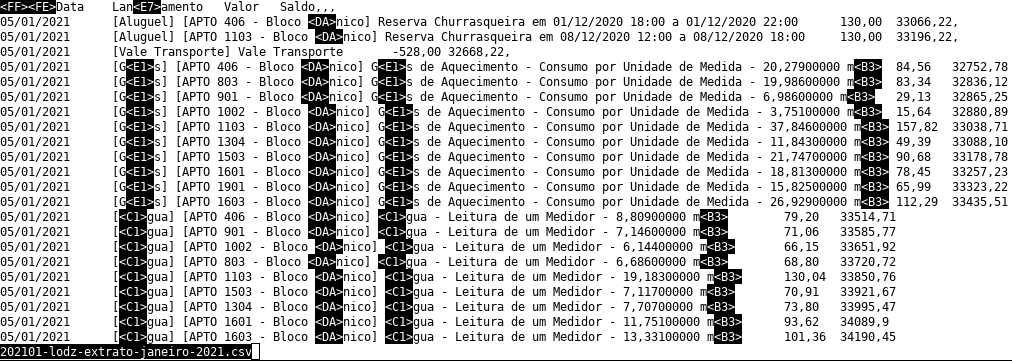
\includegraphics[width=0.8\textwidth,height=0.7\textheight,keepaspectratio]{examples/lodz-planilha-csv.png}

\framebreak
\lstinputlisting[label=lst-lodz-ex-data, postbreak=\mbox{$\hookrightarrow$\space}, basicstyle=\fontsize{5}{7}\selectfont\ttfamily]{examples/datasample.csv}

\framebreak
\lstinputlisting[language=bash, label=lst-lodz-ex-01, postbreak=\mbox{$\hookrightarrow$\space}, basicstyle=\fontsize{8}{10}\selectfont\ttfamily]{examples/analise.sh}

\framebreak
\lstinputlisting[language=bash, label=lst-lodz-ex-02, postbreak=\mbox{$\hookrightarrow$\space}, basicstyle=\fontsize{8}{10}\selectfont\ttfamily]{examples/extractdataall.sh}

\framebreak
\lstinputlisting[language=bash, label=lst-lodz-ex-03, postbreak=\mbox{$\hookrightarrow$\space}, basicstyle=\fontsize{8}{10}\selectfont\ttfamily]{examples/extractdataapto.sh}


\end{frame}



\begin{frame}
Sugestões de leitura: 
\vspace{2ex}

\fullcite{wickhamggplot2}
Disponível em: \url{https://ggplot2-book.org/}

\vspace{3ex}
From Data to Viz: \url{https://www.data-to-viz.com/}

\vspace{3ex}
The R Graph Gallery: \url{https://www.r-graph-gallery.com/}

\vspace{3ex}
Storytelling with data: \url{https://www.storytellingwithdata.com}\\
/blog, /book, /chart guide

\end{frame}

